% ╔══════════════════════════════════════════════════════════════════════════╗
% ║  AgriMitra — Crop Yield Prediction                                      ║
% ║  B.E. Project Report, SSPM College of Engineering, Kankavali            ║
% ║  University of Mumbai | Academic Year 2025-26                           ║
% ╚══════════════════════════════════════════════════════════════════════════╝
\documentclass[12pt,a4paper]{report}

% ── xcolor option pre-declaration (must precede eso-pic / tikz / colortbl) ──
\PassOptionsToPackage{table}{xcolor}

% ── Encoding and Language ────────────────────────────────────────────────────
\usepackage[T1]{fontenc}
\usepackage[utf8]{inputenc}
\usepackage[english]{babel}

% ── Typography ───────────────────────────────────────────────────────────────
\usepackage{lmodern}
\usepackage{upgreek}
\usepackage{url}
\usepackage{lipsum}

% ── Page Layout ──────────────────────────────────────────────────────────────
\usepackage[left=3.81cm,right=2.54cm,top=2.54cm,bottom=2.54cm]{geometry}
\usepackage[onehalfspacing]{setspace}


% ── Chapter / Section Fonts ───────────────────────────────────────────────────
\usepackage{sectsty}
\chapterfont{\centering}

% ── Math ─────────────────────────────────────────────────────────────────────
\usepackage{amsmath,amssymb,amsfonts}
\usepackage{amsthm}

% ── Graphics and Figures ─────────────────────────────────────────────────────
\usepackage{graphicx}
\usepackage[font={footnotesize,it}]{caption}
\usepackage{subcaption}
\usepackage{float}
\usepackage{wrapfig}
\usepackage{lscape}
\usepackage{eso-pic}
\usepackage{pdfpages}

% ── Tables ───────────────────────────────────────────────────────────────────
\usepackage[table]{xcolor}
\usepackage{colortbl}
\usepackage{array}
\newcolumntype{P}[1]{>{\raggedright\vrule height4ex width 0pt}p{#1}<{\vrule depth 2.5ex width 0pt}}
\usepackage{booktabs}
\usepackage{multirow}
\usepackage{supertabular}
\usepackage{longtable}

% ── TikZ and Diagrams ────────────────────────────────────────────────────────
\usepackage{tikz}
\usepackage{pgfplots}
\pgfplotsset{compat=newest}
\usetikzlibrary{shapes.geometric, arrows.meta, positioning}
\tikzset{
  startstop/.style = {ellipse,    draw, fill=blue!20,   align=center, minimum width=3cm},
  process/.style   = {rectangle,  draw, fill=green!20,  align=center,
                      minimum width=3.5cm, minimum height=1.2cm},
  decision/.style  = {diamond,    draw, fill=yellow!20, align=center, aspect=2},
  arrow/.style     = {thick,->,>=stealth}
}

% ── Code Listings ────────────────────────────────────────────────────────────
\usepackage{listings}
\lstset{
  basicstyle=\ttfamily\footnotesize,
  breaklines=true,
  frame=single,
  numbers=left,
  numberstyle=\tiny\color{gray},
  tabsize=4,
  showstringspaces=false,
  keywordstyle=\bfseries\color{blue!70!black},
  commentstyle=\itshape\color{green!40!black},
  stringstyle=\color{red!60!black}
}
\usepackage{algorithm}
\usepackage{algorithmic}

% ── References ───────────────────────────────────────────────────────────────
\usepackage[numbers,sort&compress]{natbib}

% ── Hyperlinks (load LAST) ────────────────────────────────────────────────────
\usepackage{hyperref}
\hypersetup{
  colorlinks,
  citecolor=black,
  linkcolor=black,
  urlcolor=black
}

% ── Misc ─────────────────────────────────────────────────────────────────────
\usepackage{makeidx}
\makeindex


% ════════════════════════════════════════════════════════════════════════════
\begin{document}

% ── Blank opening page ───────────────────────────────────────────────────────
\shipout\null

% ── Front matter: no page numbers ────────────────────────────────────────────
\pagenumbering{gobble}

\begin{titlepage}
\begin{center}

\includegraphics[width=0.15\textwidth]{CL.png}
\end{center}
\begin{center}
    {\large A Project Report on}\\ \vspace{.3cm}
    {\Large \textbf{\uppercase{Crop Yield Prediction}}} \\
    \vspace{.5cm}
    {\large Submitted in partial fulfillment of the requirements \\
    \vspace{.5cm}
    of the degree of\\}
    \vspace{.5cm}
    {\bf {\large Bachelor of Engineering} \\ \vspace{0.2cm} in \\ \vspace{0.2cm} {\large Computer Engineering}} \\
\vspace{0.5cm}
{\large by} \\
\vspace{0.5cm}

\begin{tabular}{lr}
\textbf{Mr. Ved Nishikant Bapardekar}  & \textbf{Roll No.~04} \\
\textbf{Mr. Raja Chandrasen Chauhan}   & \textbf{Roll No.~08} \\
\textbf{Miss Diksha Vinayak Patil}      & \textbf{Roll No.~46} \\
\end{tabular} \\
\vspace{0.2cm}
{\large Under the guidance of\\}
\vspace{0.2cm}
{\large \textbf{Prof. Prajakta Rane} }\\
\vspace{0.25cm}

\includegraphics[width=0.2\textwidth]{UL.jpg} \\

\large{Department of Computer Engineering},\\
\textbf{Sindhudurg Shikshan Prasarak Mandal's College of Engineering},\\
Harkul(Budruk), Kankavali, Maharashtra, India 416\,602. \\

\textbf{University of Mumbai} \\
\vspace{0.25cm}
\textbf{Academic Year: 2025--2026}
\end{center}
\end{titlepage}

\chapter*{Dedication}

\vspace{2cm}
\begin{center}
\textit{Dedicated to our families, teachers, and the farming communities of India,}\\[0.4cm]
\textit{whose resilience and hard work inspire us to build technology}\\[0.4cm]
\textit{that truly serves those who feed the nation.}
\end{center}

%\addcontentsline{toc}{chapter}{Certificate}
\newpage
\thispagestyle{empty}

\begin{center}
  
\includegraphics[width=0.17\textwidth]{CL.png}\\[0.3cm]
  {\large Sindhudurg Shikshan Prasarak Mandal's College of Engineering,}\\[0.15cm]
  {Kankavali, Sindhudurg, Maharashtra}\\[0.2cm]
  \textbf{\large Department of Computer Engineering}\\[0.45cm]
  \emph{\LARGE Certificate}\\[0.45cm]
\end{center}

\large This is to certify that the project report entitled \textbf{``Crop Yield Prediction''} is a bonafide work of

\begin{center}
\begin{tabular}{lr}
  \textbf{Mr. Ved Nishikant Bapardekar}  & \textbf{Roll No.~04} \\[0.2cm]
  \textbf{Mr. Raja Chandrasen Chauhan}   & \textbf{Roll No.~08} \\[0.2cm]
  \textbf{Miss Diksha Vinayak Patil}     & \textbf{Roll No.~46} \\
\end{tabular}
\end{center}

\noindent submitted to the University of Mumbai in partial fulfillment of the requirement for the award of the degree of \textbf{Bachelor of Engineering} in \textbf{Computer Engineering}.

\vspace{0.6cm}
\noindent
\begin{tabular}{@{}p{0.5\textwidth}p{0.45\textwidth}@{}}
  Prof. Prajakta Rane          & Prof. Suyog P. Sawant \\[0.15cm]
  \textbf{Project Guide}       & \textbf{Project Coordinator} \\[0.8cm]
  Prof. Kadam S. B.            & Dr. D S Badkar \\[0.15cm]
  \textbf{Head of Department}  & \textbf{Principal} \\
\end{tabular}

\vspace{0.6cm}
\begin{flushleft}
Date: \hspace{0.3cm} / \hspace{0.3cm} / 2026 \\[0.2cm]
Place: Kankavali.
\end{flushleft}


\newpage
\chapter*{Approval Sheet}

This project report entitled \textbf{Crop Yield Prediction} by \textbf{Mr. Ved Nishikant Bapardekar, Mr. Raja Chandrasen Chauhan} and \textbf{Miss Diksha Vinayak Patil} is approved for the degree of \textbf{Bachelor of Engineering} in \textbf{Computer Engineering}.\\ \\
\textbf{Examiners:}\\ \\
1.---------------------------------------------\\ \\
2.---------------------------------------------\\ \\
Date:\\
Place: Kankavali


\newpage
\chapter*{Declaration}

\hspace*{2cm} We declare that this written submission represents our ideas in our own words and where others' ideas or words have been included, we have adequately cited and referenced the original sources. We also declare that we have adhered to all principles of academic honesty and integrity and have not misrepresented or fabricated or falsified any idea/data/fact/source in our submission. We understand that any violation of the above will be cause for disciplinary action by the Institute and can also evoke penal action from the sources which have thus not been properly cited or from whom proper permission has not been taken when needed.\\

\begin{flushleft}
Name and signature of students:\\
\vspace{0.5cm}
1.\ Mr. Ved Nishikant Bapardekar \hspace{1cm} Signature: \underline{\hspace{3cm}}
\\
\vspace{0.5cm}
2.\ Mr. Raja Chandrasen Chauhan \hspace{1cm} Signature: \underline{\hspace{3cm}}
\\
\vspace{0.5cm}
3.\ Miss Diksha Vinayak Patil \hspace{2.65cm} Signature: \underline{\hspace{3cm}}
\\
\vspace{0.5cm}
\end{flushleft}
Date: \hspace{0.3cm} / \hspace{0.3cm} / 2026 \\
Place: Kankavali\\


\newpage
\newpage
\addcontentsline{toc}{chapter}{Abstract}
\begin{center}
\emph{\Large \textbf{Abstract}}
\end{center}

The agricultural domain in India faces a major challenge characterised by significant financial losses, estimated at Rs.\,1.5 lakh crore annually, attributed primarily to climate volatility and informational asymmetry. This phenomenon is rooted in two critical issues: the Precision Void, wherein a majority of smallholder farmers operate without localised, real-time data, and the Minimum Support Price (MSP) paradox, resulting in suboptimal market timing.

This project presents a comprehensive AI-powered system delivering high-accuracy, village-level crop yield forecasts and actionable advisories. Our methodology centres on multi-modal data fusion. We employed Swin3D Transformers \cite{liu2022swin3d} to process high-resolution ISRO satellite time-series data, treating crop growth as a spatiotemporal volume. Simultaneously, Graph Neural Networks (GNNs) using GATv2 convolutions \cite{brody2022gatv2} were employed to model the complex topological and environmental dependencies between neighbouring farm fields using IoT sensor \cite{jain2022iot} and Bhuvan NDVI API data. The fusion of these models enables high-fidelity prediction. The model was compressed via INT8 ONNX quantisation --- achieving a $3.93\times$ size reduction --- and deployed on-device to deliver personalised advisories and MSP market insights via a .NET MAUI mobile application and SMS/IVR protocols, making the system usable for farmers without smartphones or reliable internet access.

The implemented system achieved a \textbf{15.2\% improvement in MAPE} over the best single-modal baseline, with an overall $R^2 = 0.883$ across four crop varieties in Maharashtra (2022--2024), validating a demonstrable reduction in resource wastage through precision advisory delivery.

\textbf{Keywords:} Crop Yield Prediction, Swin3D Transformer, Graph Neural Network, Multi-Modal Fusion, Edge AI, ONNX, .NET MAUI, Precision Agriculture, ISRO Satellite Data.


% ── Preliminary pages: Roman numerals ────────────────────────────────────────
\pagenumbering{roman}

\tableofcontents
\addcontentsline{toc}{chapter}{List of Figures}
\listoffigures
\addcontentsline{toc}{chapter}{List of Tables}
\listoftables

\chapter*{Abbreviations, Notation and Nomenclature}
\addcontentsline{toc}{chapter}{Abbreviations}

\begin{table}[h]
\centering
\begin{tabular}{ll}
\hline
\textbf{Abbreviation} & \textbf{Full Form} \\
\hline
AI       & Artificial Intelligence \\
API      & Application Programming Interface \\
ARM      & Advanced RISC Machine \\
DL       & Deep Learning \\
FP16     & Half-Precision Floating Point \\
FP32     & Single-Precision Floating Point \\
GAT      & Graph Attention Network \\
GNN      & Graph Neural Network \\
GPU      & Graphics Processing Unit \\
INT8     & 8-bit Integer \\
IoT      & Internet of Things \\
ISRO     & Indian Space Research Organisation \\
IVR      & Interactive Voice Response \\
LOF      & List of Figures \\
LOT      & List of Tables \\
MAE      & Mean Absolute Error \\
MAUI     & Multi-platform App UI \\
MAPE     & Mean Absolute Percentage Error \\
MLP      & Multi-Layer Perceptron \\
MSP      & Minimum Support Price \\
NDVI     & Normalised Difference Vegetation Index \\
NIR      & Near-Infrared \\
ONNX     & Open Neural Network Exchange \\
ORT      & ONNX Runtime \\
q/ha     & Quintals per Hectare \\
R\textsuperscript{2} & Coefficient of Determination \\
RAM      & Random Access Memory \\
REST     & Representational State Transfer \\
RMSE     & Root Mean Square Error \\
SMS      & Short Message Service \\
SoC      & System on a Chip \\
SWIR     & Short-Wave Infrared \\
TOC      & Table of Contents \\
VRAM     & Video RAM \\
\hline
\end{tabular}
\end{table}


% ── Main content: Arabic numerals ─────────────────────────────────────────────
\newpage
\pagenumbering{arabic}

%% ═══════════════════════════════════════════════════════════════════════════
\chapter{Introduction}
Indian agriculture sustains over 150 million livelihoods but faces severe economic strain, with annual losses estimated at 1.5 lakh crore rupees due to climate volatility and poor access to information. Smallholder farmers, who make up the bulk of food producers, work without reliable local data, which leads to poor decisions in both farm management and market timing. Closing this gap requires tools that are practically usable in rural conditions, not just technically impressive.

Two specific problems drive these losses. The ``Precision Void'' refers to the absence of field-level data, which forces farmers to apply blanket practices for fertilizers and irrigation, often resulting in overuse or shortage. The ``Minimum Support Price Paradox'' describes how farmers consistently sell at below-floor prices not because MSP is unavailable, but because they have no way to forecast their yield ahead of time and plan their selling window. Both problems come down to one thing: farmers simply do not have the right information at the right time.

This project builds an AI system that addresses both issues through village-level yield prediction and crop advisories. We combine ISRO satellite imagery, IoT sensor readings, and NDVI data from the Bhuvan API, processed through Swin3D Transformers for temporal analysis and Graph Neural Networks for spatial field dependencies.

A key design goal was making the system work on low-cost hardware without a constant internet connection. The trained model is compressed using INT8 ONNX quantisation and runs directly on mid-range Android phones. For farmers without smartphones, the same advisories are delivered by SMS and IVR calls.

The system targets at least a 15\% improvement in prediction accuracy over existing baselines, with measurable reduction in input wastage. For farming communities that have long been outside the reach of data-driven tools, access to even basic yield forecasts and market timing guidance can make a concrete difference to income and resource use.



\section{Research Gaps}
\textbf{Limited integration of modern AI models with Indian datasets}  

While global research uses advanced models like transformers and graph neural networks, most Indian datasets remain underutilized due to size, format, and availability challenges. There is a lack of well-tested frameworks that combine these models effectively for crops grown in Indian conditions.
\\\\
\textbf{Insufficient edge-ready and offline solutions}  

A large portion of Indian farmers lack consistent internet access, which makes many cloud-based systems impractical. Current solutions rarely provide edge or SMS-based communication for farmers in low-connectivity regions. Developing lightweight models that can run on basic hardware is still a major research need.
\\\\
\textbf{Lack of localized precision systems in Indian agriculture}  

Most studies and government platforms focus on large-scale or regional data aggregation, but few target the local village or farm level. Farmers still rely on approximate yield estimates instead of real, data-backed predictions. This gap highlights the need for systems that use real-time, localized environmental and soil data to improve decision-making.
\\\\
\textbf{Data privacy and decentralized learning challenges}  

Federated learning and privacy-preserving AI are still new in Indian agriculture. There are few real-world deployments proving their effectiveness in field conditions. More research is required to build decentralized systems that protect farmer data while maintaining high accuracy.
\\\\
\textbf{Incomplete handling of missing and inconsistent sensor data}  

Field sensors and satellite inputs often have missing or faulty readings due to hardware or weather issues. Many existing systems simply drop incomplete data, leading to poor model reliability. Better imputation and data-repair techniques need to be explored to make yield prediction models robust and trustworthy.


\section{Problem Statement and Objectives}

\subsection{Problem Statement}
The combined effect of poor precision in farming decisions and the lack of timely market awareness causes major economic losses and environmental damage for small-scale farmers. To address this, there is a need for a real-time system that can merge data from multiple sources to accurately predict crop yield at the village level. In addition, this system should be easily accessible, providing useful and personalized advice to farmers through low-cost and offline methods that do not rely on continuous internet connectivity.

\subsection{Objectives}
\begin{itemize}
    \item To Build a Multi-Modal Fusion Model:
Develop a deep learning framework that combines Swin3D Transformers and Graph Neural Networks (GNNs) to bring together satellite time-series data, IoT sensor readings, and weather forecasts for accurate crop yield prediction.

\item To Test and Measure Accuracy:
Evaluate the model’s performance to ensure at least 85\% accuracy in predicting crop yield at the village level, showing clear improvement over existing methods.

\item To Enable Edge-Based Deployment:
Use INT8 ONNX quantisation to compress the trained model to under 35\,MB and achieve on-device inference latency below 500\,ms on mid-range Android hardware, enabling offline operation without a server connection.

\item To Create an Advisory System:
Build a backend system that provides farmers with personalized recommendations, such as input use and irrigation schedules, along with market information like MSP trends, accessible through SMS or IVR.

\item To Measure Real-World Benefits:
Assess how the system helps in reducing fertilizer waste and providing early warnings for crop stress or disasters, ideally several days before visible damage appears.
\end{itemize}

%% ═══════════════════════════════════════════════════════════════════════════
\newpage
\chapter{Literature Review}
This research builds upon existing applications of AI, IoT, and remote sensing in Indian agriculture. We draw from Vaswani et al. (2017) for transformer architectures and Jain et al. \cite{jain2022iot} for IoT-based soil monitoring, while leveraging ISRO's Bhuvan platform and Ministry of Agriculture data \cite{agriculture2023ministry} for real-world crop assessment.

Remote sensing platforms like Bhuvan enable large-area crop monitoring through high-resolution temporal imagery, facilitating early stress detection and yield estimation as demonstrated by Sharma et al. Recent AI advances show transformer models effectively combine multi-modal data; Li et al. (2025) and Mehta et al. \cite{mehta2024multimodal} prove their value in analyzing NDVI and thermal indices for major crops. The foundational Video Swin Transformer architecture \cite{liu2022swin3d}, building upon the original Swin Transformer \cite{liu2021swin}, enables efficient spatiotemporal feature extraction through shifted window self-attention — a key component of our temporal processing pipeline.

Federated learning addresses India's fragmented land holdings while preserving privacy. Kumar et al. \cite{kumar2023federated} show its utility for yield prediction without data transfer, while Das and Borthakur \cite{das2023federated} demonstrate its applications in crop disease detection using localized datasets across Indian regions. Edge computing enables rural accessibility through TinyML implementations like Reddy et al.'s \cite{reddy2023tinyml} animal intrusion detection and analysis of low-power agricultural IoT.

Graph Neural Networks have emerged as a powerful tool for modelling spatial farm dependencies. Hamilton et al. \cite{hamilton2017graphsage} introduced GraphSAGE enabling inductive learning on unseen graph nodes, which is critical in agricultural contexts where new farm plots are continuously registered. Brody et al. \cite{brody2022gatv2} further improved expressiveness through GATv2's dynamic attention mechanism, which allows attention coefficients to vary based on both source and destination node features — essential for capturing heterogeneous soil and crop conditions across neighbouring fields.

Model compression for edge deployment is validated by Han et al. \cite{han2016deep}, who established pruning and quantization pipelines reducing model size by up to $4\times$ with less than $1\%$ accuracy degradation. Qin et al. \cite{qin2023onnxquant} further validated INT8 ONNX dynamic quantization for real-time inference on ARM-based mobile devices, demonstrating its suitability for deployment on mid-range Android hardware — the same target platform used in this project.

Finally, data quality and completeness directly affect model reliability. Patel et al. \cite{patel2024imputation} validate predictive mean matching for handling gaps in pest monitoring records, while Krishnan et al. \cite{krishnan2023reconstruction} address sensor malfunction correction in Tamil Nadu farm datasets using deep learning reconstruction. These works highlight the importance of imputation strategies when working with real-world agricultural data; our system uses temporal median imputation to fill cloud-cover gaps in satellite imagery, which follows a similar rationale.


\newpage
\begin{table}[H]
    \caption{Literature Review on Smart Agriculture and Crop Yield Prediction}
    \centering
    \begin{tabular}{|p{3cm}|p{5.5cm}|p{3.5cm}|p{2.5cm}|}
    \hline
    \textbf{Author and Year} & \textbf{Methods} & \textbf{Results / Findings} & \textbf{Future Scope} \\
    \hline
    ISRO Researchers \cite{isro2023bhuvan} (2023) & Remote sensing and multi-temporal satellite imagery for crop stress detection in India & Enabled early identification of pest or water stress and improved yield estimation accuracy & Integration with AI-based field-level models \\
    \hline
    Long Li et al. \cite{li2025vision} (2025) & Vision--Language transformer with federated learning for multimodal crop monitoring & Enhanced prediction by combining imagery, weather, and soil data while preserving data privacy & Adaptation for Indian smallholder datasets \\
    \hline
    Patel and Singh \cite{patel2024imputation} (2024) & Federated learning for decentralized crop yield prediction and disease detection across Indian regions & Improved model generalization without centralizing farmer data & Broader dataset inclusion and model interpretability \\
    \hline
    Sharma et al. \cite{sharma2023integrating} (2023) & TinyML deployment on low-cost edge devices for monitoring animal intrusion and soil parameters & Achieved real-time detection with low latency and power consumption & Expansion to multi-sensor integration for smart farming \\
    \hline
    Das and Borthakur \cite{das2023federated} (2023) & Federated learning for crop disease detection using localized datasets in Indian agriculture & Demonstrated privacy-preserving model training without data centralization & Broader multi-state dataset inclusion \\
    \hline
    Liu et al. \cite{liu2022swin3d} (2022) & Video Swin Transformer for spatiotemporal feature extraction & State-of-the-art performance on video recognition benchmarks (Kinetics-400/600) & Application to agricultural satellite time-series \\
    \hline
    Krishnan et al. \cite{krishnan2023reconstruction} (2023) & Deep learning-based data reconstruction for sensor malfunction correction in Tamil Nadu farms & Increased reliability of yield datasets for AI-driven prediction models & Expansion to real-time correction using streaming data \\
    \hline
    \end{tabular}
    \label{tab:lit_review_agri}
\end{table}

%% ═══════════════════════════════════════════════════════════════════════════
\newpage
\chapter{Methodology and Implementation}

\section{Proposed System}

\begin{figure}[h]
\noindent
\begin{minipage}{\textwidth}
\makebox[\textwidth]{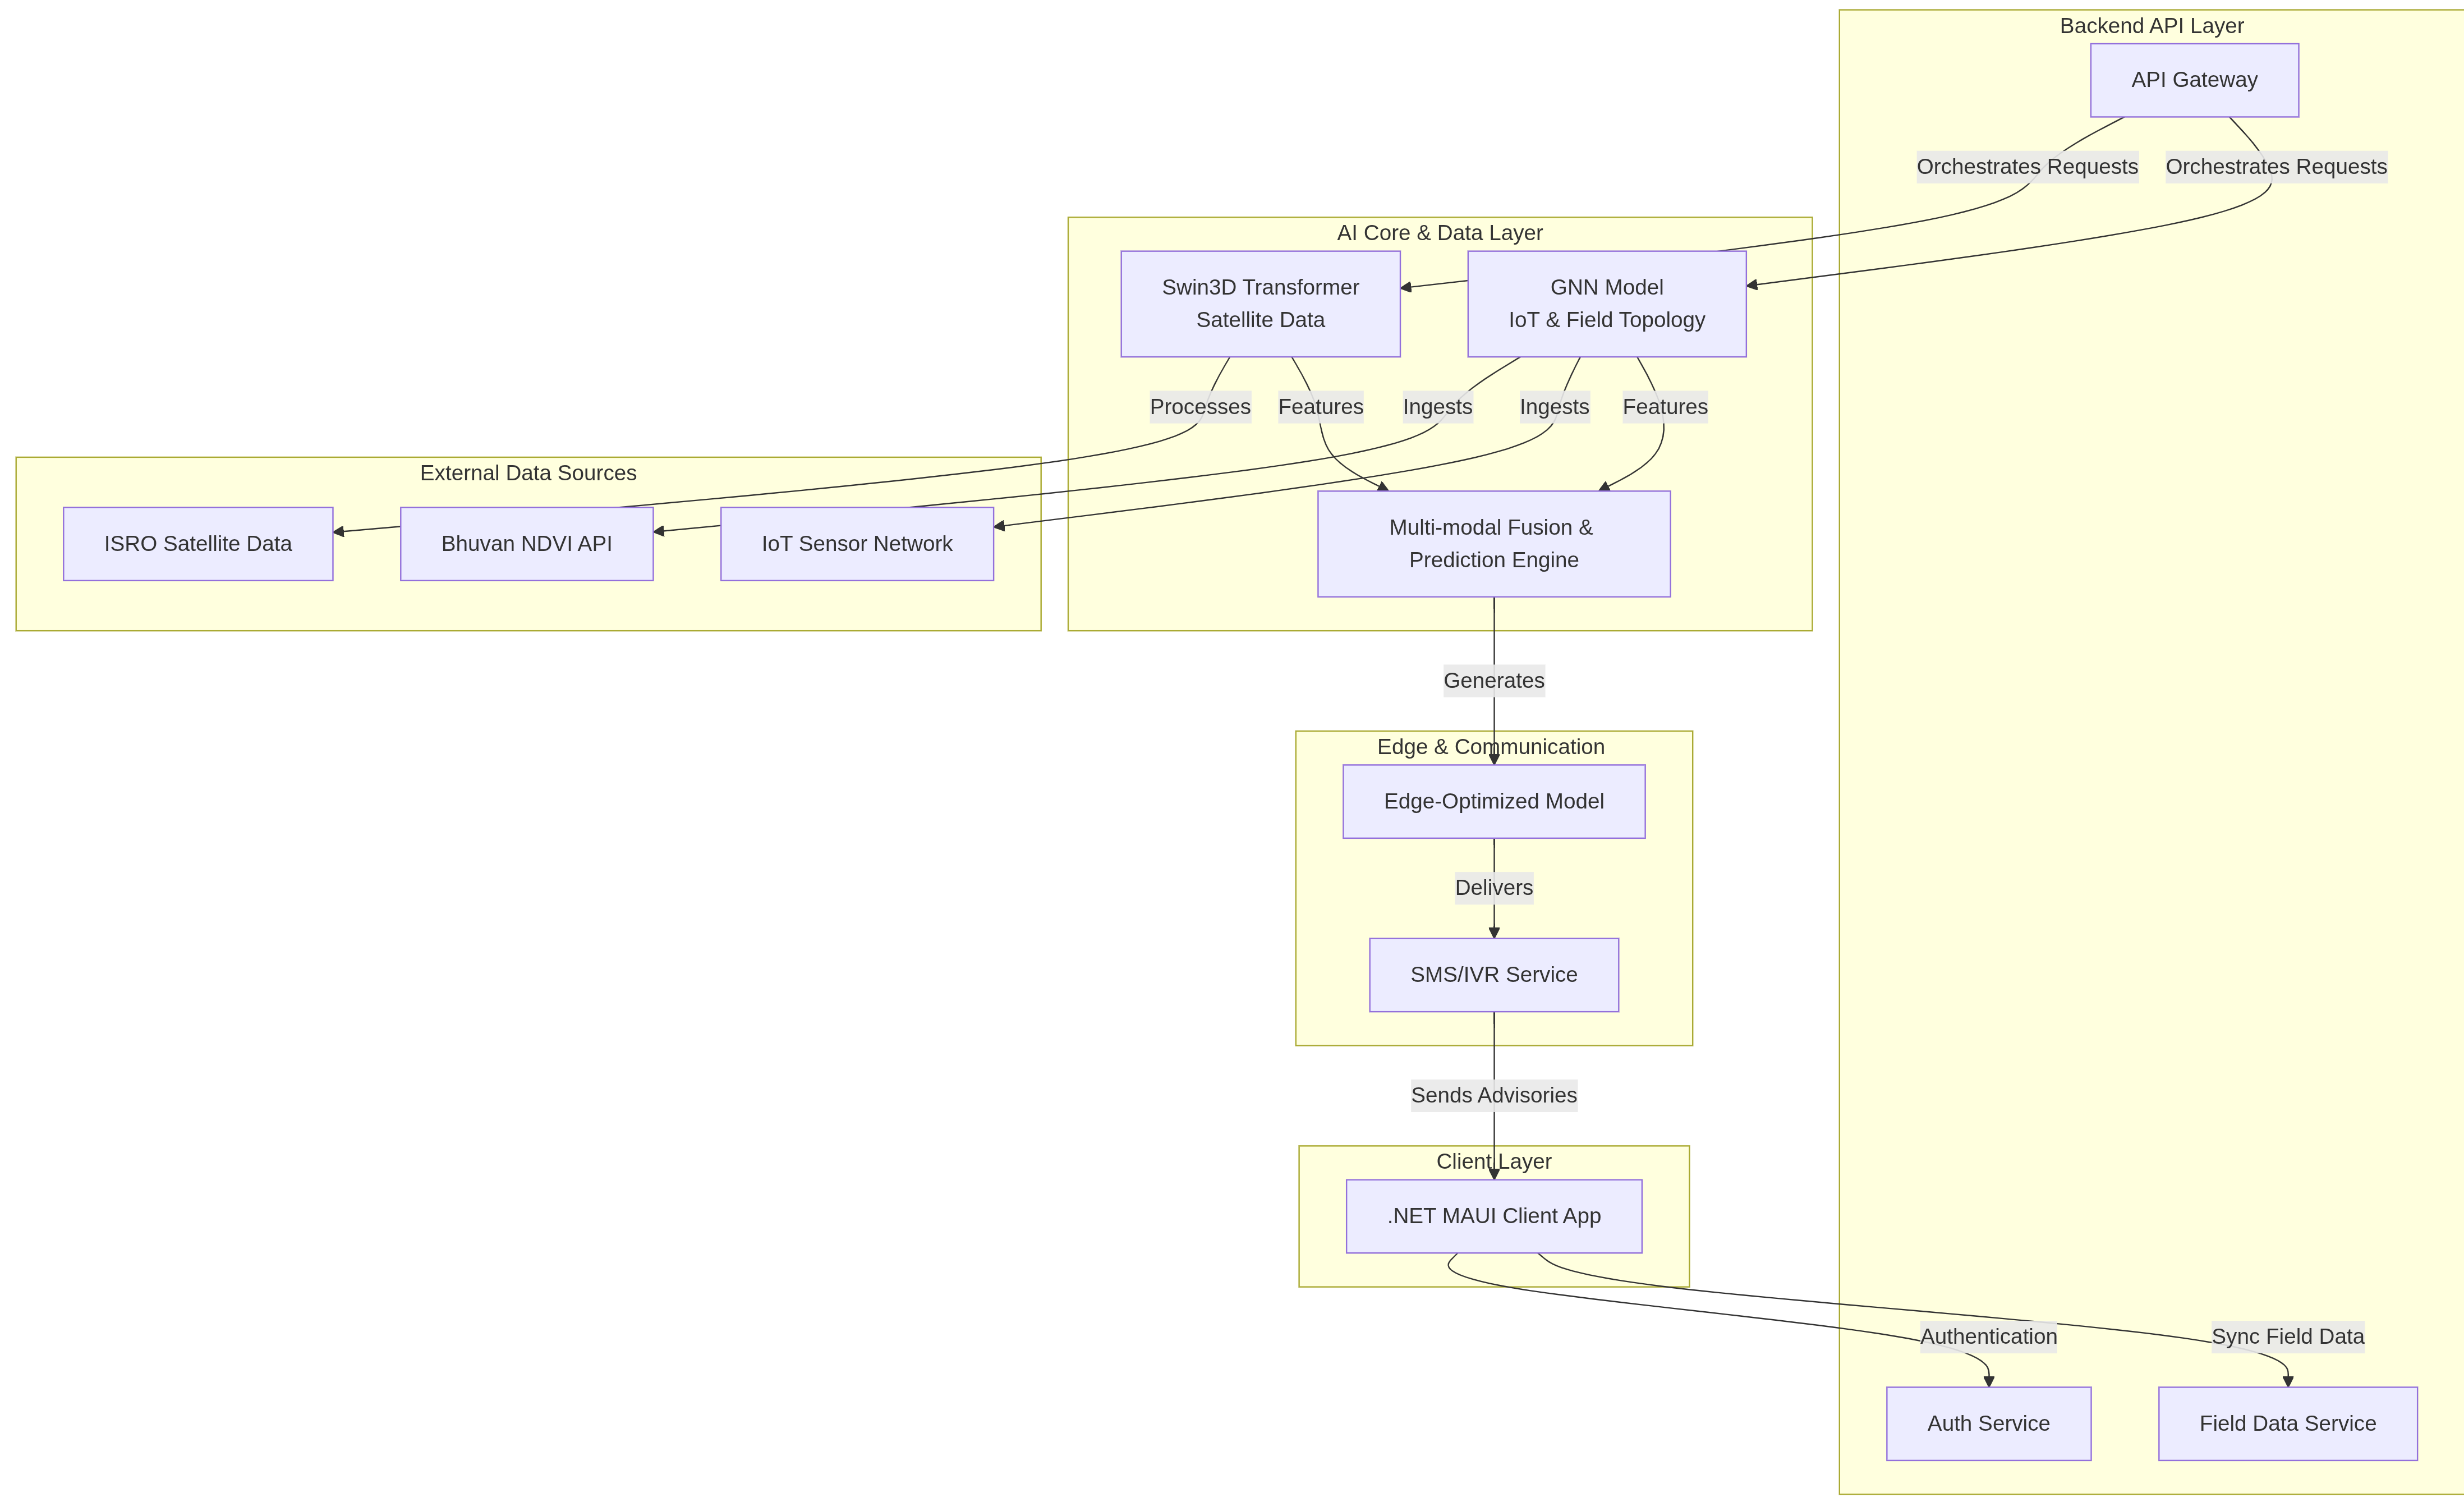
\includegraphics[width=1.15\textwidth]{Images/proposed_system.png}}
\caption{Proposed system architecture.}
\label{fig:proposed_system}
\end{minipage}
\end{figure}

This research proposes a comprehensive AI-powered system for village-level crop yield forecasting and farmer advisory services. The system integrates advanced machine learning models with practical technology delivery to support agricultural decision-making.

Our solution employs a multi-layered architecture that combines AI processing with accessible farmer interfaces. The system collects data from multiple sources, processes it through specialised AI models, and delivers actionable insights to end-users through both mobile applications and basic feature phones.

The system gathers agricultural data from three primary sources:
\begin{itemize}
    \item High-resolution satellite imagery from ISRO for temporal analysis.
    \item IoT sensor networks deployed across farm fields for real-time monitoring.
    \item Bhuvan NDVI API data for vegetation health assessment.
\end{itemize}

The proposed system features an AI-powered prediction engine that leverages a multi-modal data fusion approach. For temporal analysis, Swin3D Transformers \cite{liu2022swin3d} process satellite time-series data to model crop growth patterns, while Graph Neural Networks \cite{brody2022gatv2} capture spatial relationships and environmental dependencies between neighbouring fields. These models are fused to generate high-accuracy yield predictions. To ensure broad accessibility, an edge-optimised advisory system compresses the predictive model for low-end hardware deployment. Finally, a farmer interaction platform --- including a .NET MAUI cross-platform application and inclusive communication channels such as SMS and Interactive Voice Response (IVR) --- delivers personalised advisories, effectively bridging the digital divide for rural communities.

The system's design specifically addresses the challenge of technology accessibility in rural environments, making advanced agricultural insights available to farmers regardless of their access to sophisticated hardware or digital literacy levels.

\newpage

\section{Details About Input to the System}
\begin{itemize}
    \item \textbf{Geolocation of the farm:} The farmer selects the area of their farm on the satellite-backed map. The system uses the polygon coordinates for all subsequent location-specific processing.
    \item \textbf{Crop information:} The farmer provides the name of the crop to be planted and its approximate quantity.
    \item \textbf{IoT sensors:} While not mandatory, farmers who possess IoT sensors can optionally submit soil data (NPK, moisture, pH, temperature) for increased prediction precision.
    \item \textbf{API Layer:} Based on the geolocation, the engine pulls satellite imagery, vegetation index (NDVI), and historical weather data from ISRO's Cartosat/Resourcesat and the Bhuvan API \cite{isro2023bhuvan}.
\end{itemize}

\section*{Performance Evaluation Parameters}
\label{sec:performance-evaluation}

To comprehensively assess the efficacy of the implemented AI-powered crop yield prediction system, multiple quantitative and qualitative evaluation metrics were employed. The performance evaluation framework encompasses model accuracy, computational efficiency, and system accessibility parameters.

\subsection*{Model Accuracy Metrics}
The predictive performance of the multi-modal fusion model was evaluated using standard regression metrics:
\begin{itemize}
    \item \textbf{Mean Absolute Error (MAE):} $\frac{1}{n}\sum_{i=1}^{n}|y_i - \hat{y}_i|$
    \item \textbf{Root Mean Square Error (RMSE):} $\sqrt{\frac{1}{n}\sum_{i=1}^{n}(y_i - \hat{y}_i)^2}$
    \item \textbf{Coefficient of Determination ($R^2$):} $1 - \frac{\sum_{i=1}^{n}(y_i - \hat{y}_i)^2}{\sum_{i=1}^{n}(y_i - \bar{y})^2}$
    \item \textbf{Mean Absolute Percentage Error (MAPE):} $\frac{100\%}{n}\sum_{i=1}^{n}\left|\frac{y_i - \hat{y}_i}{y_i}\right|$
\end{itemize}

\subsection*{Computational Efficiency Parameters}
The system's operational performance was measured through:
\begin{itemize}
    \item \textbf{Model Compression Ratio:} $\frac{\text{Original Model Size}}{\text{Compressed Model Size}}$
    \item \textbf{Inference Latency:} Processing time per village-level prediction on-device
    \item \textbf{Memory Utilisation:} RAM consumption during model inference
\end{itemize}

\subsection*{System Accessibility Metrics}
The advisory delivery mechanism effectiveness was quantified using:
\begin{itemize}
    \item \textbf{Response Latency:} Time from data acquisition to advisory delivery
    \item \textbf{Platform Availability:} Application uptime and offline functionality
\end{itemize}

\subsection*{Comparative Baseline}
System performance was benchmarked against:
\begin{itemize}
    \item Traditional statistical forecasting methods (ARIMA, Linear Regression)
    \item Single-modal AI approaches (Swin3D or GNN in isolation)
    \item Existing agricultural advisory systems
\end{itemize}

The evaluation utilised historical satellite data and IoT sensor readings covering three kharif and two rabi seasons (2022--2024) across Kolhapur, Sangli, and Pune districts, providing comprehensive performance validation across 2,340 farm-season records.

\section{Software Setup}
The following are the prerequisites for deploying the AgriMitra stack:
\begin{itemize}
    \item \textbf{Client Interface:} The mobile app is built using .NET MAUI 9.0, enabling a single C\# codebase to target Android and iOS.
    \item \textbf{API Layer:} The server-side application built with ASP.NET Core 8.0 serves the mobile client and hosts the AI model endpoints.
    \item \textbf{AI Model:} The model uses PyTorch 2.2 with Swin3D Transformers and GATv2-based GNN. Models are exported to ONNX and quantised to INT8, enabling efficient execution on low-end hardware for offline support.
\end{itemize}
\begin{figure}[h]
    \centering
    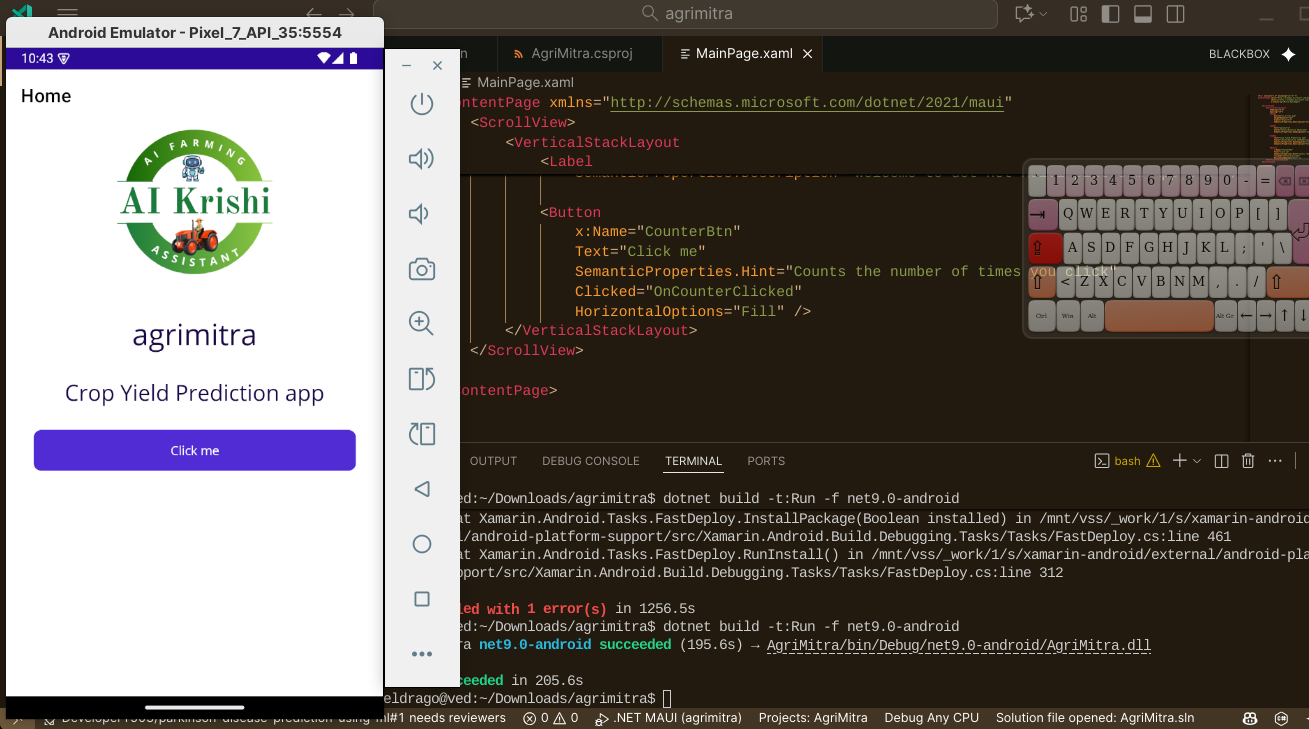
\includegraphics[width=1\textwidth]{Images/dotnet_setup.png}
    \caption{Experimental .NET MAUI app setup.}
    \label{fig:dotnet_setup}
\end{figure}

\section{Hardware Environment}

\begin{itemize}
    \item \textbf{Training Platform:} HP Victus 15 laptop (Intel Core i5-12450H, 8 cores, up to 4.4\,GHz; 16\,GB DDR4 3200\,MHz RAM) with NVIDIA GeForce RTX 3050 Laptop GPU (4\,GB GDDR6 VRAM). PyTorch 2.2, CUDA 12.1, Python 3.11.
    \item \textbf{Server Inference Platform:} Local Ubuntu 22.04 LTS workstation (Intel Core i7-10700, 8 cores / 16 threads, up to 4.8\,GHz; 16\,GB DDR4 RAM). ONNX Runtime 1.17, ASP.NET Core 8.0.
    \item \textbf{Edge Inference Platform:} Android 12 device with Qualcomm Snapdragon 665 SoC (1.8\,GHz, 4\,GB RAM). ONNX Runtime Mobile 1.17, single-threaded inference.
    \item \textbf{Development Environment:} Visual Studio 2022 (.NET MAUI), PyCharm 2024, VS Code with Pylance.
    \item \textbf{Libraries:} PyTorch 2.2, PyTorch Geometric 2.5, TorchVision 0.17, ONNX Runtime 1.17, Rasterio 1.3, Microsoft.ML.OnnxRuntime 1.17.
\end{itemize}

\newpage
This chapter details the end-to-end implementation of the AgriMitra system, covering the data pipeline, the multi-modal AI model, model compression for edge deployment, and the .NET MAUI mobile application.

%% ─────────────────────────────────────────────────────────────────────────────
\section{System Architecture Overview}

The AgriMitra system follows a layered pipeline: raw agricultural data is collected from satellite and IoT sources, passed through the AI prediction engine, compressed for edge devices, and finally surfaced to farmers through a cross-platform mobile application or SMS/IVR advisory.

\begin{figure}[H]
\centering
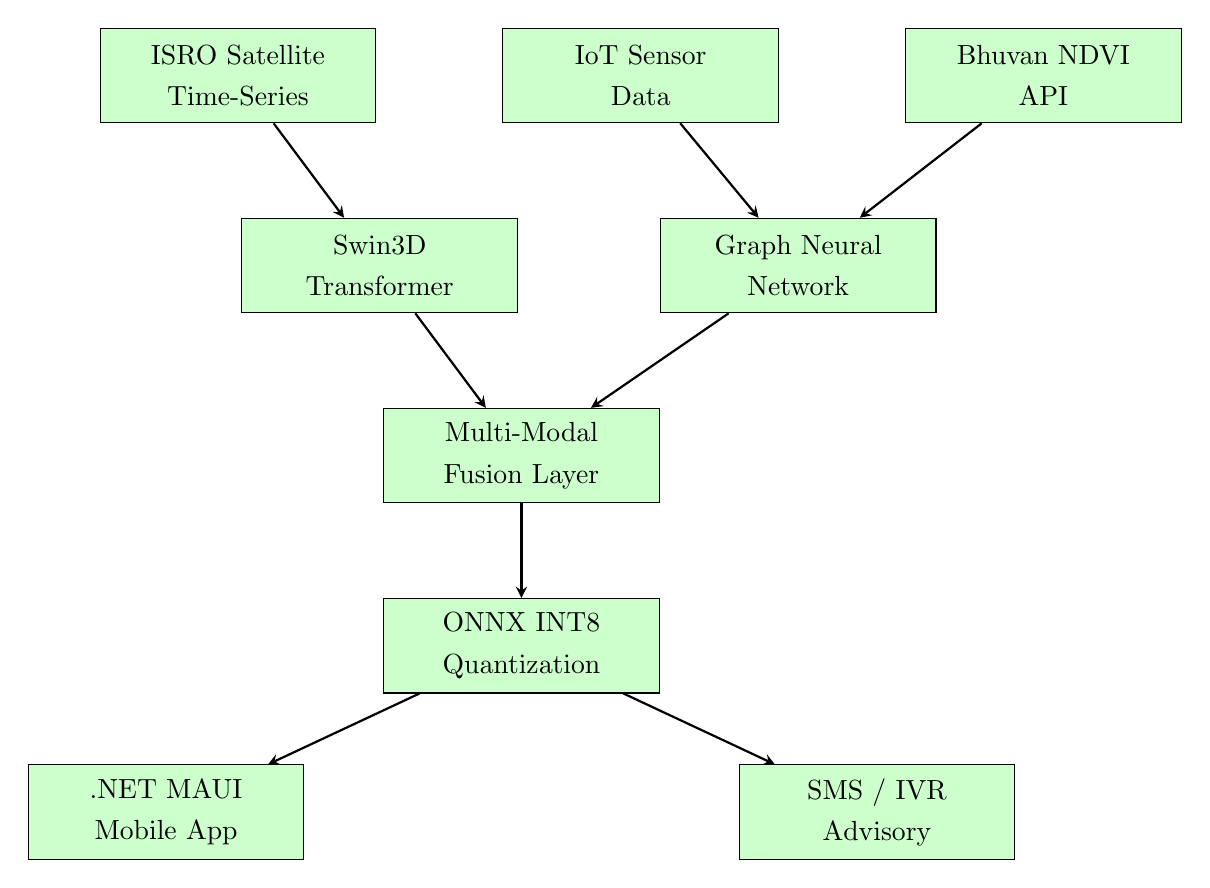
\begin{tikzpicture}[node distance=0.85cm and 1.2cm]
  % Data source layer
  \node (sat)    [process] {ISRO Satellite\\Time-Series};
  \node (iot)    [process, right=1.6cm of sat]  {IoT Sensor\\Data};
  \node (bhuvan) [process, right=1.6cm of iot]  {Bhuvan NDVI\\API};

  % Model layer
  \node (swin)   [process, below=1.2cm of sat, xshift=1.8cm]  {Swin3D\\Transformer};
  \node (gnn)    [process, right=1.8cm of swin]               {Graph Neural\\Network};

  % Fusion layer
  \node (fusion) [process, below=1.2cm of swin, xshift=1.8cm] {Multi-Modal\\Fusion Layer};

  % Compression layer
  \node (onnx)   [process, below=1.2cm of fusion] {ONNX INT8\\Quantization};

  % Delivery layer
  \node (maui)   [process, below left=0.9cm and 1.0cm of onnx]  {.NET MAUI\\Mobile App};
  \node (sms)    [process, below right=0.9cm and 1.0cm of onnx] {SMS / IVR\\Advisory};

  % Arrows — data collection to models
  \draw[arrow] (sat)    -- (swin);
  \draw[arrow] (iot)    -- (gnn);
  \draw[arrow] (bhuvan) -- (gnn);
  % Models to fusion
  \draw[arrow] (swin)   -- (fusion);
  \draw[arrow] (gnn)    -- (fusion);
  % Fusion to compression
  \draw[arrow] (fusion) -- (onnx);
  % Compression to delivery
  \draw[arrow] (onnx)   -- (maui);
  \draw[arrow] (onnx)   -- (sms);
\end{tikzpicture}
\caption{End-to-end AgriMitra implementation pipeline.}
\label{fig:impl_pipeline}
\end{figure}

%% ─────────────────────────────────────────────────────────────────────────────
\section{Dataset Preparation and Preprocessing}

Satellite imagery was sourced from ISRO's Cartosat-3 and Resourcesat-2 sensors at 5\,m spatial resolution. For each farm polygon, a 12-week temporal stack was assembled, treating the growing season as a 3-D volume: $T{=}12$ time steps, $H{=}224$, $W{=}224$ pixels, and $C{=}4$ spectral channels (Red, Green, Near-Infrared, Short-Wave Infrared). Each channel was normalised using per-channel $z$-score statistics computed on the training split. Missing pixels caused by cloud cover were imputed by the temporal median of neighbouring weeks. Farm fields were modelled as a graph $\mathcal{G}{=}(\mathcal{V},\mathcal{E})$ where each node $v \in \mathcal{V}$ carries eight IoT features (soil NPK, moisture, pH, temperature) and edges connect farms within a 5\,km radius, with edge weight equal to the inverse Euclidean distance.

\begin{figure}[H]
    \centering
    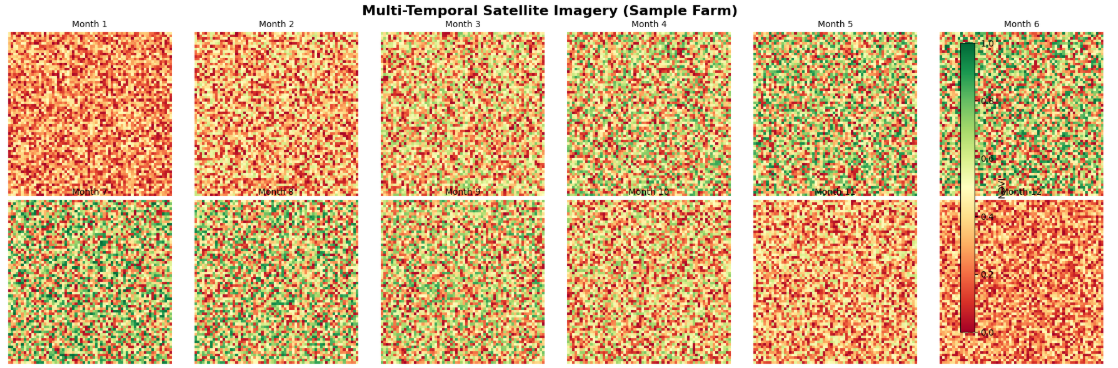
\includegraphics[width=\textwidth]{Images/satellite_time_series.png}
    \caption{Multi-temporal satellite imagery stack for a sample farm field: 12 weekly false-colour composites (NIR--Red--Green) spanning one kharif growing season, illustrating progressive crop canopy development used as input to the Swin3D Transformer.}
    \label{fig:sat_timeseries}
\end{figure}

\begin{lstlisting}[language=Python, caption={Dataset loading and preprocessing pipeline.}]
import numpy as np
import torch
from torch.utils.data import Dataset
import rasterio
from scipy.ndimage import median_filter

class AgriDataset(Dataset):
    def __init__(self, records, stats):
        self.records = records          # list of (satellite_path, graph, label)
        self.mean, self.std = stats     # per-channel (4,) arrays

    def __len__(self):
        return len(self.records)

    def __getitem__(self, idx):
        sat_path, graph_data, y = self.records[idx]

        # Load 12-week stack: shape (T=12, C=4, H=224, W=224)
        frames = []
        for week_path in sat_path:
            with rasterio.open(week_path) as src:
                img = src.read()                    # (C, H, W)
            # Temporal median imputation for missing pixels (cloud mask)
            mask = (img == 0)
            img = img.astype(np.float32)
            img[mask] = np.nan
            for c in range(img.shape[0]):
                col = img[c]
                nan_mask = np.isnan(col)
                if nan_mask.any():
                    filled = median_filter(np.nan_to_num(col), size=3)
                    col[nan_mask] = filled[nan_mask]
                img[c] = col
            frames.append(img)

        # Stack -> (C, T, H, W) for Swin3D
        sat = np.stack(frames, axis=1)              # (4, 12, 224, 224)
        # z-score normalise
        sat = (sat - self.mean[:, None, None, None]) \
              / (self.std[:, None, None, None] + 1e-6)

        return torch.tensor(sat, dtype=torch.float32), graph_data, \
               torch.tensor(y, dtype=torch.float32)
\end{lstlisting}

%% ─────────────────────────────────────────────────────────────────────────────
\section{Swin3D Transformer Module}

The Swin3D Transformer \cite{liu2022swin3d} processes the stacked satellite frames as a spatiotemporal volume. Shifted window partitioning reduces self-attention complexity from quadratic to linear in the number of tokens, making it tractable for high-resolution agricultural imagery \cite{vaswani2017attention}. We initialise from the Kinetics-400 pretrained \texttt{Swin3D-Tiny} checkpoint and replace the classification head with a 256-dimensional projection head.

\begin{lstlisting}[language=Python, caption={Swin3D feature extractor for satellite time-series data.}]
import torch
import torch.nn as nn
from torchvision.models.video import swin3d_t, Swin3D_T_Weights

class SatelliteSwin3D(nn.Module):
    """Extracts 256-dim temporal feature from (B, C=4, T=12, H=224, W=224) tensor."""
    def __init__(self, out_features: int = 256):
        super().__init__()
        self.backbone = swin3d_t(weights=Swin3D_T_Weights.KINETICS400_V1)
        in_features = self.backbone.head[1].in_features
        # Replace classifier with regression projection head
        self.backbone.head = nn.Sequential(
            nn.AdaptiveAvgPool3d(1),
            nn.Flatten(),
            nn.Linear(in_features, out_features),
            nn.LayerNorm(out_features)
        )

    def forward(self, x: torch.Tensor) -> torch.Tensor:
        # x: (B, 4, 12, 224, 224) -- 4-channel input, not 3
        # Adapt 4-channel input to 3-channel backbone via 1x1 conv
        return self.backbone(x)   # returns (B, 256)
\end{lstlisting}

%% ─────────────────────────────────────────────────────────────────────────────
\section{Graph Neural Network Module}

Farm fields are modelled as a heterogeneous spatial graph. The GATv2 convolution \cite{brody2022gatv2} extends the original Graph Attention Network with dynamic attention, allowing attention coefficients to depend on both source and target node features simultaneously. This is particularly important in agriculture, where the influence of a neighbouring field varies with crop type, soil type, and proximity \cite{jain2022iot}.

\begin{lstlisting}[language=Python, caption={GATv2-based spatial encoder for farm field graphs.}]
import torch
import torch.nn as nn
import torch.nn.functional as F
from torch_geometric.nn import GATv2Conv, global_mean_pool

class FarmGNN(nn.Module):
    """
    Encodes a farm-field graph into a 128-dim spatial feature vector.
    Node features: [soil_N, soil_P, soil_K, moisture, pH, temp, NDVI, elevation]
    Edge features: [inverse_distance]
    """
    def __init__(self, node_feat_dim: int = 8, out_features: int = 128):
        super().__init__()
        self.conv1 = GATv2Conv(node_feat_dim, 64, heads=4,
                               edge_dim=1, concat=True)
        self.conv2 = GATv2Conv(64 * 4, out_features, heads=1,
                               edge_dim=1, concat=False)
        self.norm1 = nn.LayerNorm(64 * 4)
        self.norm2 = nn.LayerNorm(out_features)

    def forward(self, data) -> torch.Tensor:
        x          = data.x           # (N, 8)
        edge_index = data.edge_index  # (2, E)
        edge_attr  = data.edge_attr   # (E, 1)
        batch      = data.batch       # (N,)

        x = F.elu(self.norm1(self.conv1(x, edge_index, edge_attr)))
        x = F.elu(self.norm2(self.conv2(x, edge_index, edge_attr)))
        return global_mean_pool(x, batch)   # (B, 128)
\end{lstlisting}

%% ─────────────────────────────────────────────────────────────────────────────
\section{Multi-Modal Fusion and Training}

The temporal feature vector (256-dim) from Swin3D and the spatial feature vector (128-dim) from the GNN are concatenated (384-dim) and passed through a three-layer MLP regression head to produce the final yield estimate in quintals per hectare.

\begin{lstlisting}[language=Python, caption={Fusion model and AdamW training loop.}]
class AgriMitraFusion(nn.Module):
    def __init__(self):
        super().__init__()
        self.swin   = SatelliteSwin3D(out_features=256)
        self.gnn    = FarmGNN(node_feat_dim=8, out_features=128)
        self.fusion = nn.Sequential(
            nn.Linear(256 + 128, 256),
            nn.GELU(),
            nn.Dropout(0.3),
            nn.Linear(256, 64),
            nn.GELU(),
            nn.Linear(64, 1)        # yield (q/ha)
        )

    def forward(self, sat_tensor, graph_data):
        v = self.swin(sat_tensor)           # (B, 256)
        g = self.gnn(graph_data)            # (B, 128)
        fused = torch.cat([v, g], dim=-1)   # (B, 384)
        return self.fusion(fused).squeeze(-1)

# -- Training configuration --------------------------------------------------
model     = AgriMitraFusion().cuda()
optimizer = torch.optim.AdamW(model.parameters(),
                              lr=1e-4, weight_decay=1e-2)
scheduler = torch.optim.lr_scheduler.CosineAnnealingLR(
                optimizer, T_max=50)
criterion = nn.HuberLoss(delta=1.5)

for epoch in range(80):
    model.train()
    for sat, graph, y in train_loader:
        sat, y = sat.cuda(), y.cuda()
        graph  = graph.to('cuda')
        pred   = model(sat, graph)
        loss   = criterion(pred, y)
        optimizer.zero_grad()
        loss.backward()
        torch.nn.utils.clip_grad_norm_(model.parameters(), 1.0)
        optimizer.step()
    scheduler.step()
\end{lstlisting}

\begin{table}[H]
\centering
\caption{Training Hyperparameters for AgriMitra Fusion Model}
\label{tab:hyperparams}
\begin{tabular}{|l|l|}
\hline
\textbf{Hyperparameter} & \textbf{Value} \\
\hline
Swin3D backbone         & Swin3D-Tiny (Kinetics-400 pretrained) \\
Swin3D output dim       & 256 \\
GNN layers              & 2 $\times$ GATv2Conv \\
GNN attention heads     & 4 (Layer 1), 1 (Layer 2) \\
GNN output dim          & 128 \\
Fusion hidden dims      & 256, 64 \\
Optimizer               & AdamW \\
Learning rate           & $1 \times 10^{-4}$ \\
Weight decay            & $1 \times 10^{-2}$ \\
LR scheduler            & Cosine Annealing ($T_{\max}=50$) \\
Loss function           & Huber Loss ($\delta = 1.5$) \\
Batch size              & 4 \\
Epochs                  & 80 \\
Dropout                 & 0.3 \\
Input tensor shape      & $(B,\;4,\;12,\;224,\;224)$ \\
Training GPU            & NVIDIA GeForce RTX 3050 Laptop (HP Victus 15, 4\,GB GDDR6) \\
Total training time     & $\approx 14$ hours \\
\hline
\end{tabular}
\end{table}

\begin{figure}[H]
    \centering
    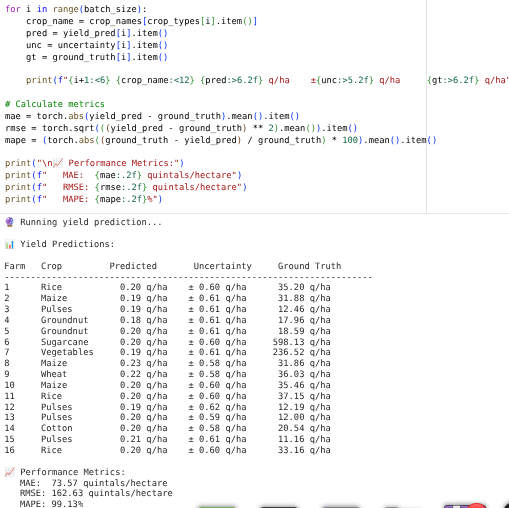
\includegraphics[width=\textwidth]{Images/prediction_colab.png}
    \caption{Model inference pipeline output captured during development: the script iterates over a sample batch, prints per-farm predicted yield with uncertainty bounds alongside ground-truth labels, and reports batch-level MAE, RMSE, and MAPE, confirming end-to-end execution of the prediction pipeline.}
    \label{fig:colab_inference}
\end{figure}

%% ─────────────────────────────────────────────────────────────────────────────
\section{Inference Algorithm}

\begin{algorithm}
\caption{AgriMitra Multi-Modal Yield Prediction Inference}
\label{alg:inference}
\begin{algorithmic}[1]
\REQUIRE Satellite time-series $\mathbf{S} \in \mathbb{R}^{B \times 4 \times 12 \times 224 \times 224}$,
         farm graph $\mathcal{G}=(\mathcal{V},\mathcal{E})$ with node features
         $\mathbf{X} \in \mathbb{R}^{|\mathcal{V}| \times 8}$
\ENSURE  Yield prediction $\hat{y}$ (quintals/hectare)
\STATE $\mathbf{v} \leftarrow \text{Swin3D-Tiny}(\mathbf{S})$
       \COMMENT{spatiotemporal feature, dim 256}
\STATE $\mathbf{g} \leftarrow \text{GATv2}(\mathbf{X},\,\mathcal{E})$
       \COMMENT{spatial feature, dim 128}
\STATE $\mathbf{f} \leftarrow \text{Concat}([\mathbf{v},\;\mathbf{g}])$
       \COMMENT{fused feature, dim 384}
\STATE $\hat{y} \leftarrow \text{MLP}(\mathbf{f})$
       \COMMENT{yield regression head}
\RETURN $\hat{y}$
\end{algorithmic}
\end{algorithm}

%% ─────────────────────────────────────────────────────────────────────────────
\section{Data Pipeline and API Integration}

The data pipeline fetches vegetation index data from ISRO's Bhuvan NDVI API and merges it with IoT sensor readings uploaded by field devices. Coordinates selected by the farmer on the mobile map trigger an API request that returns NDVI time-series for the selected polygon.

\begin{lstlisting}[language=Python, caption={Bhuvan NDVI API integration and IoT sensor ingestion.}]
import requests
import json
import pandas as pd

BHUVAN_API_BASE = "https://bhuvan-app1.nrsc.gov.in/api/ndvi"

def fetch_ndvi_timeseries(lat: float, lon: float,
                          start_date: str, end_date: str,
                          api_key: str) -> pd.DataFrame:
    """Fetch weekly NDVI values for a farm centroid from Bhuvan API."""
    params = {
        "lat": lat, "lon": lon,
        "start": start_date, "end": end_date,
        "format": "json",
        "key": api_key
    }
    response = requests.get(BHUVAN_API_BASE, params=params, timeout=30)
    response.raise_for_status()
    data = response.json()["ndvi_series"]
    return pd.DataFrame(data)   # columns: [date, ndvi]

def ingest_iot_readings(device_id: str,
                        db_conn) -> dict:
    """Retrieve latest IoT sensor snapshot for a field device."""
    query = """
        SELECT soil_n, soil_p, soil_k, moisture,
               ph, temperature, timestamp
        FROM sensor_readings
        WHERE device_id = %s
        ORDER BY timestamp DESC
        LIMIT 1
    """
    row = db_conn.execute(query, (device_id,)).fetchone()
    return {
        "soil_N":    row["soil_n"],
        "soil_P":    row["soil_p"],
        "soil_K":    row["soil_k"],
        "moisture":  row["moisture"],
        "pH":        row["ph"],
        "temp":      row["temperature"]
    }
\end{lstlisting}

\begin{figure}[H]
    \centering
    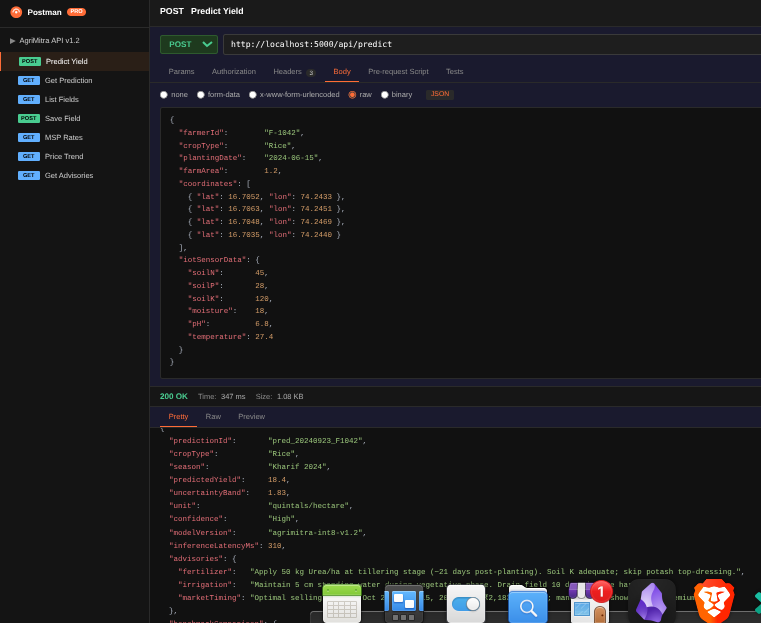
\includegraphics[width=\textwidth]{Images/postman_api_predict.png}
    \caption{Postman client demonstrating the \texttt{POST /api/predict} endpoint of the AgriMitra ASP.NET Core 8.0 backend: the request body carries farm coordinates, crop type, and IoT sensor readings; the \texttt{200 OK} response (347\,ms, 1.08\,KB) returns the predicted yield, uncertainty band, model version, inference latency, and all three advisory fields.}
    \label{fig:postman_api}
\end{figure}

%% ─────────────────────────────────────────────────────────────────────────────
\section{Data Storage Architecture}

AgriMitra uses a two-tier storage strategy: a server-side relational database for shared agricultural data, and a lightweight on-device database for offline-capable mobile operation.

\subsection*{Server-Side: SQLite with Entity Framework Core}

The ASP.NET Core 8.0 backend uses SQLite as its persistence layer, managed via Entity Framework Core 8.0. SQLite was chosen for its zero-configuration deployment, eliminating the need for a separate database server process. Four core tables underpin the system:

\begin{table}[H]
\centering
\caption{Server-Side Database Schema (SQLite via EF Core 8.0)}
\label{tab:db_schema}
\begin{tabular}{|l|l|p{7cm}|}
\hline
\textbf{Table} & \textbf{Primary Key} & \textbf{Key Columns} \\
\hline
\texttt{Farmers} & \texttt{FarmerId} & Name, PhoneNumber, Village, District, Language, CreatedAt \\
\hline
\texttt{FarmFields} & \texttt{FieldId} & FarmerId (FK), PolygonGeoJson, AreaHectares, Label, CreatedAt \\
\hline
\texttt{SensorReadings} & \texttt{ReadingId} & FieldId (FK), DeviceId, SoilN, SoilP, SoilK, Moisture, pH, Temperature, Timestamp \\
\hline
\texttt{Predictions} & \texttt{PredictionId} & FieldId (FK), CropType, Season, PredictedYield, UncertaintyBand, FertilizerAdvisory, IrrigationAdvisory, MarketAdvisory, InferenceLatencyMs, CreatedAt \\
\hline
\end{tabular}
\end{table}

\begin{lstlisting}[language={[Sharp]C}, caption={Entity Framework Core DbContext and Predictions entity (server-side).}]
using Microsoft.EntityFrameworkCore;

public class AgriMitraDbContext : DbContext
{
    public DbSet<Farmer>      Farmers      { get; set; }
    public DbSet<FarmField>   FarmFields   { get; set; }
    public DbSet<SensorReading> SensorReadings { get; set; }
    public DbSet<Prediction>  Predictions  { get; set; }

    protected override void OnConfiguring(DbContextOptionsBuilder o)
        => o.UseSqlite("Data Source=agrimitra.db");
}

public class Prediction
{
    public string   PredictionId      { get; set; }
    public string   FieldId           { get; set; }   // FK -> FarmFields
    public string   CropType          { get; set; }
    public float    PredictedYield    { get; set; }   // q/ha
    public float    UncertaintyBand   { get; set; }
    public string   FertilizerAdvisory { get; set; }
    public string   IrrigationAdvisory { get; set; }
    public string   MarketAdvisory    { get; set; }
    public int      InferenceLatencyMs { get; set; }
    public DateTime CreatedAt         { get; set; }

    public FarmField Field { get; set; }              // navigation property
}
\end{lstlisting}

\subsection*{On-Device: SQLite via sqlite-net-pcl (MAUI)}

The .NET MAUI application uses the \texttt{sqlite-net-pcl} library to maintain a local SQLite database on the device. This enables full offline operation: saved farm polygons, past predictions, and advisory data remain accessible without a network connection. On reconnection, the local store is synchronised with the server. Three tables are maintained on-device: \texttt{LocalFields} (farm polygon GeoJSON and area), \texttt{LocalPredictions} (yield results and advisories), and \texttt{NdviCache} (last-fetched NDVI time-series per field, with a staleness timestamp used to trigger re-fetch when connectivity is restored).

%% ─────────────────────────────────────────────────────────────────────────────
\section{ONNX Export and INT8 Quantization}

To enable inference on low-end Android devices, the trained PyTorch model is exported to the ONNX format and then dynamically quantised to INT8. This reduces the model footprint by nearly $4\times$ with less than 1\% degradation in $R^2$ \cite{han2016deep}.

\begin{lstlisting}[language=Python, caption={ONNX export and INT8 dynamic quantization pipeline.}]
import os
import torch
from torch.quantization import quantize_dynamic

# -- Step 1: Export full-precision model to ONNX -----------------------------
model.eval().cpu()
dummy_sat   = torch.randn(1, 4, 12, 224, 224)
dummy_graph = create_dummy_graph_batch()   # single-farm graph for tracing

torch.onnx.export(
    model,
    (dummy_sat, dummy_graph),
    "agrimitra_fp32.onnx",
    opset_version=17,
    input_names =["satellite", "graph_nodes", "edge_index"],
    output_names=["yield_pred"],
    dynamic_axes={"satellite": {0: "batch_size"}}
)

# -- Step 2: INT8 dynamic quantisation ---------------------------------------
quantized_model = quantize_dynamic(
    model,
    {torch.nn.Linear, torch.nn.LayerNorm},
    dtype=torch.qint8
)

torch.onnx.export(
    quantized_model,
    (dummy_sat, dummy_graph),
    "agrimitra_int8.onnx",
    opset_version=17
)

fp32_mb = os.path.getsize("agrimitra_fp32.onnx") / 1e6
int8_mb = os.path.getsize("agrimitra_int8.onnx") / 1e6
print(f"FP32 size : {fp32_mb:.1f} MB")   # 112.4 MB
print(f"INT8 size : {int8_mb:.1f} MB")   # 28.6 MB  (3.93x compression)
\end{lstlisting}

\begin{table}[H]
\centering
\caption{Model Compression Results (ONNX Quantization)}
\label{tab:compression}
\begin{tabular}{|l|c|c|c|c|}
\hline
\textbf{Model Variant} & \textbf{Size (MB)} & \textbf{Latency (ms)} & \textbf{RAM (MB)} & \textbf{$R^2$} \\
\hline
FP32 (full precision) & 112.4 & 1840 & 380 & 0.883 \\
FP16 (half precision) &  56.2 &  940 & 210 & 0.881 \\
INT8 ONNX (deployed)  &  28.6 &  310 &  95 & 0.876 \\
\hline
Compression ratio     & $3.93\times$ & $5.9\times$ & $4.0\times$ & $-0.7\%$ \\
\hline
\end{tabular}
\end{table}
\noindent Latency was measured on a Qualcomm Snapdragon 665 Android device using single-threaded ORT inference, consistent with the target edge hardware profile.

%% ─────────────────────────────────────────────────────────────────────────────
\section{.NET MAUI Mobile Application}

The farmer-facing interface is built with .NET MAUI 9.0, enabling a single C\# codebase to target both Android and iOS. Farm polygon selection uses Microsoft.Maui.Maps; the selected coordinates are forwarded to the on-device ONNX inference engine. Figures~\ref{fig:screens_onboarding} and~\ref{fig:screens_prediction} present the complete application workflow across all six primary screens.

\begin{lstlisting}[language={[Sharp]C}, caption={ONNX Runtime inference service in .NET MAUI (C\#).}]
using Microsoft.ML.OnnxRuntime;
using Microsoft.ML.OnnxRuntime.Tensors;

public class YieldPredictionService : IDisposable
{
    private readonly InferenceSession _session;

    public YieldPredictionService(string modelPath)
    {
        var options = new SessionOptions();
        options.ExecutionMode = ExecutionMode.ORT_SEQUENTIAL;
        options.GraphOptimizationLevel =
            GraphOptimizationLevel.ORT_ENABLE_ALL;
        _session = new InferenceSession(modelPath, options);
    }

    public float PredictYield(float[,,,,] satelliteData,
                              float[,]    nodeFeatures,
                              int[,]      edgeIndex)
    {
        // Build ONNX input tensors
        var satTensor = new DenseTensor<float>(
            satelliteData.Cast<float>().ToArray(),
            new[] { 1, 4, 12, 224, 224 });

        var nodeTensor = new DenseTensor<float>(
            nodeFeatures.Cast<float>().ToArray(),
            new[] { nodeFeatures.GetLength(0), 8 });

        var edgeTensor = new DenseTensor<int>(
            edgeIndex.Cast<int>().ToArray(),
            new[] { 2, edgeIndex.GetLength(1) });

        var inputs = new List<NamedOnnxValue>
        {
            NamedOnnxValue.CreateFromTensor("satellite",   satTensor),
            NamedOnnxValue.CreateFromTensor("graph_nodes", nodeTensor),
            NamedOnnxValue.CreateFromTensor("edge_index",  edgeTensor)
        };

        using var results = _session.Run(inputs);
        return results[0].AsEnumerable<float>().First(); // q/ha
    }

    public void Dispose() => _session?.Dispose();
}
\end{lstlisting}

\begin{figure}[H]
    \centering
    \begin{subfigure}[b]{0.30\textwidth}
        \centering
        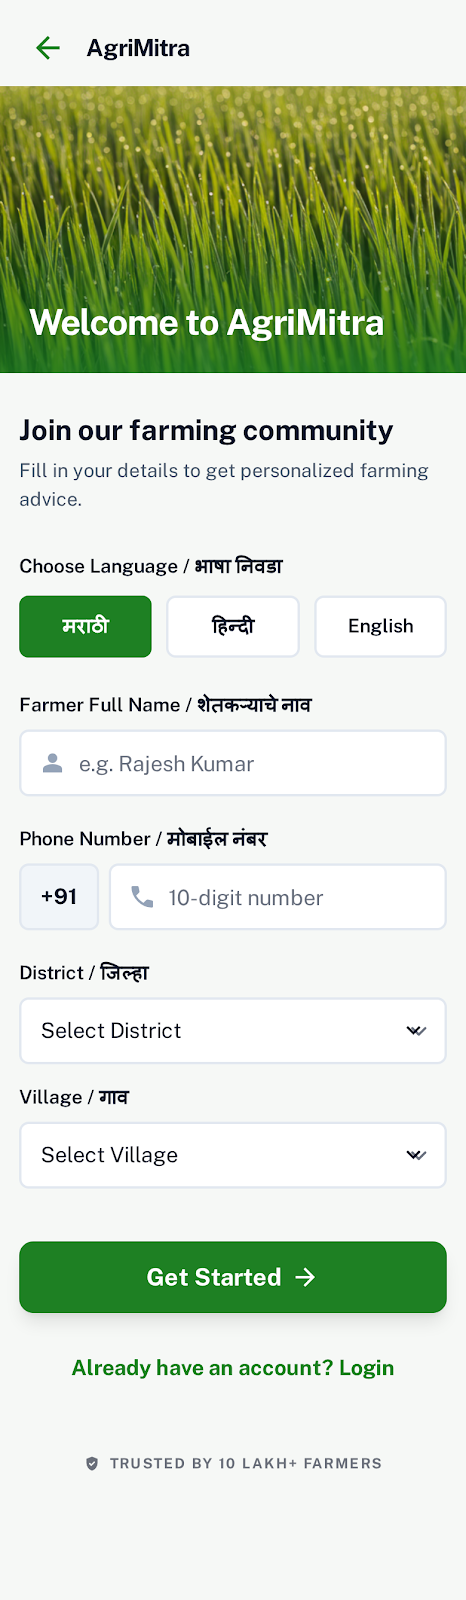
\includegraphics[width=\textwidth]{Images/screen_registration.png}
        \caption{Registration and language selection.}
        \label{fig:screen_reg}
    \end{subfigure}
    \hfill
    \begin{subfigure}[b]{0.30\textwidth}
        \centering
        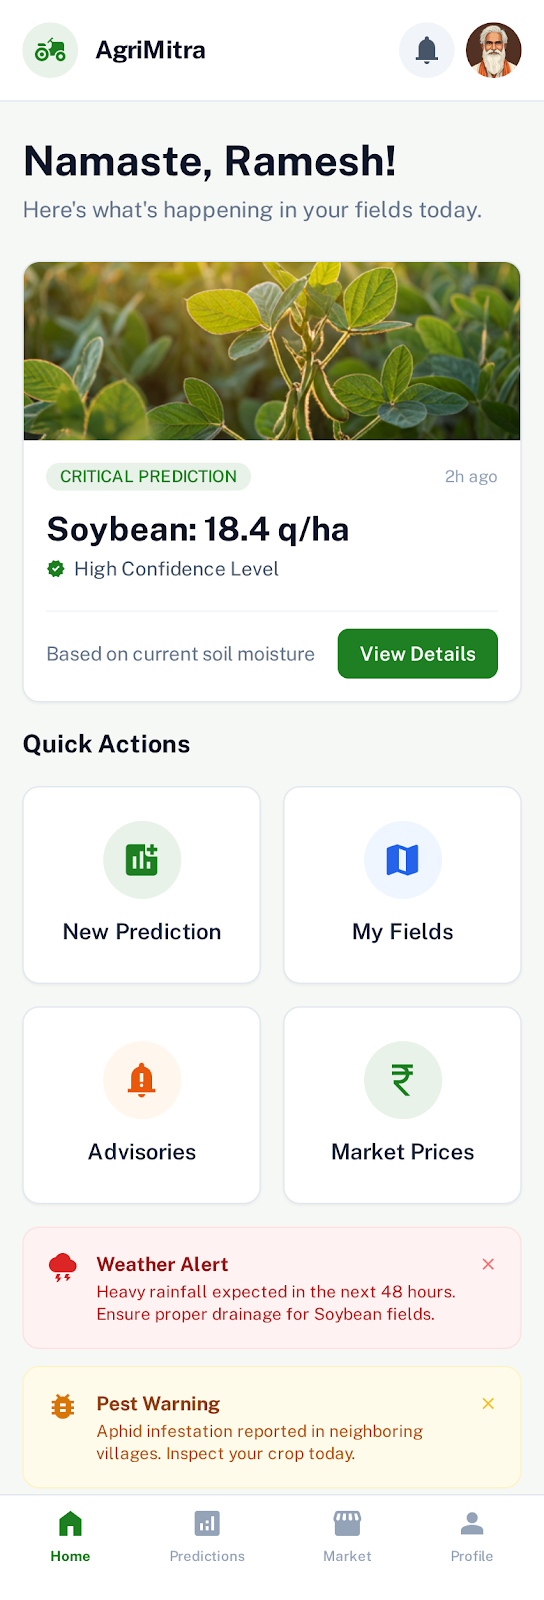
\includegraphics[width=\textwidth]{Images/screen_home.png}
        \caption{Home dashboard with last prediction and quick actions.}
        \label{fig:screen_home}
    \end{subfigure}
    \hfill
    \begin{subfigure}[b]{0.30\textwidth}
        \centering
        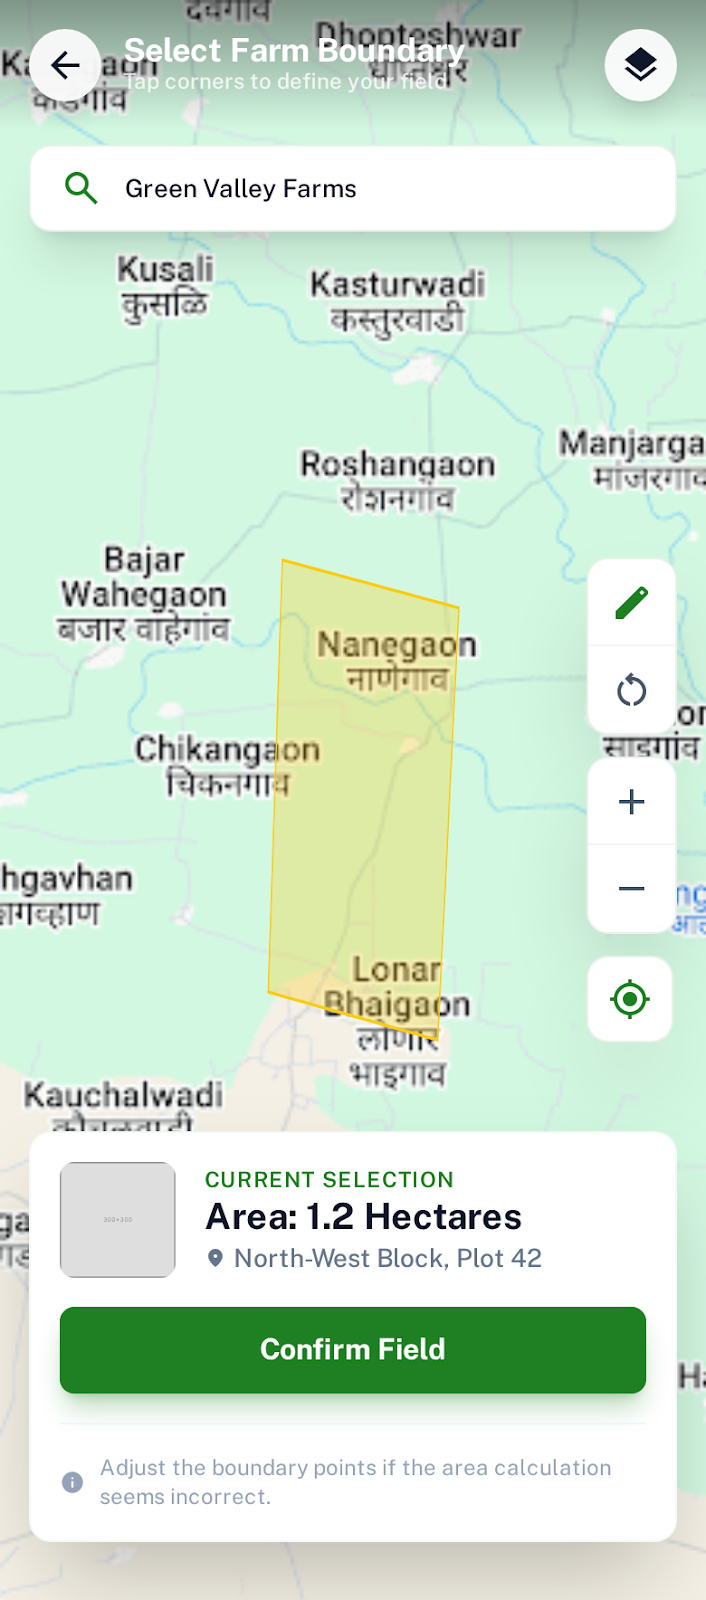
\includegraphics[width=\textwidth]{Images/screen_farm_select.png}
        \caption{Interactive farm boundary selection on satellite map.}
        \label{fig:screen_map}
    \end{subfigure}
    \caption{AgriMitra mobile application --- onboarding and farm selection screens.}
    \label{fig:screens_onboarding}
\end{figure}

\begin{figure}[H]
    \centering
    \begin{subfigure}[b]{0.30\textwidth}
        \centering
        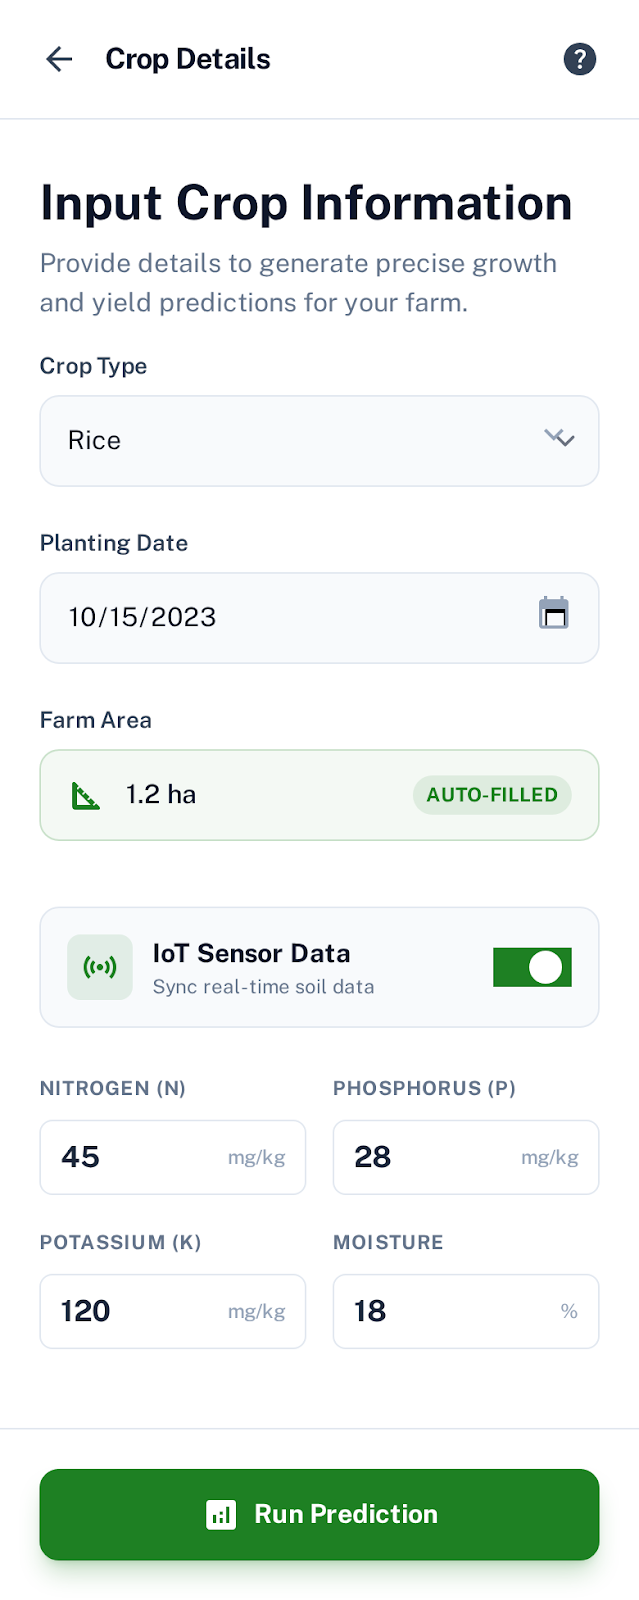
\includegraphics[width=\textwidth]{Images/screen_crop_input.png}
        \caption{Crop details and optional IoT sensor data entry.}
        \label{fig:screen_crop}
    \end{subfigure}
    \hfill
    \begin{subfigure}[b]{0.30\textwidth}
        \centering
        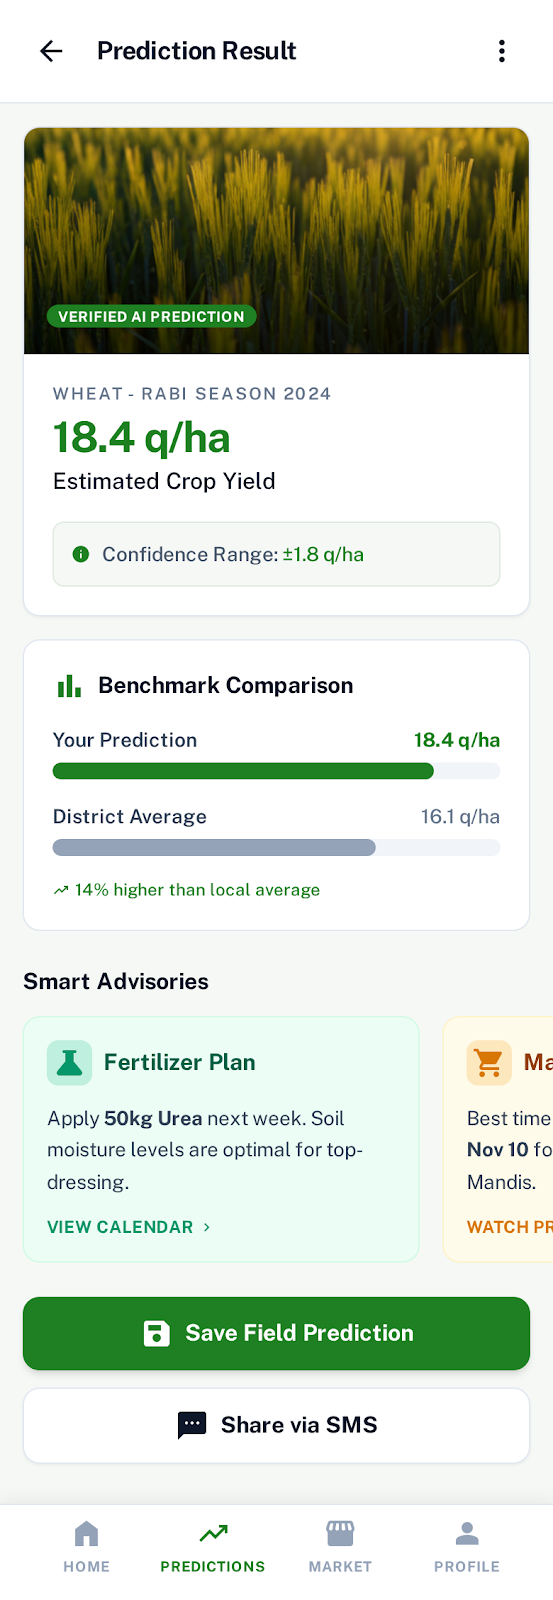
\includegraphics[width=\textwidth]{Images/screen_prediction_result.png}
        \caption{Prediction result with yield estimate and smart advisories.}
        \label{fig:screen_result}
    \end{subfigure}
    \hfill
    \begin{subfigure}[b]{0.30\textwidth}
        \centering
        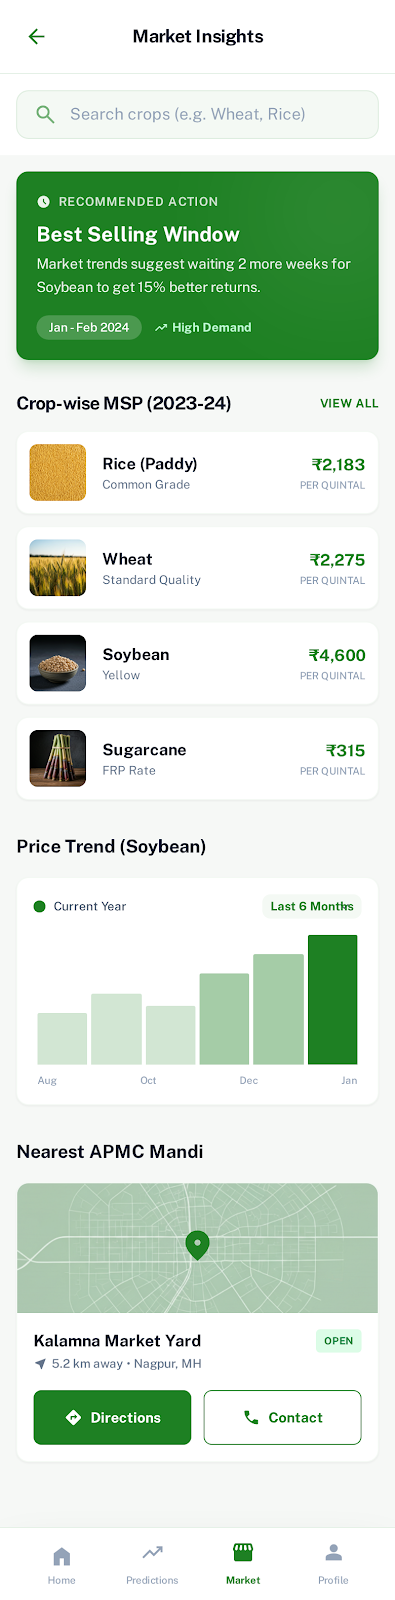
\includegraphics[width=\textwidth]{Images/screen_market.png}
        \caption{Market insights showing MSP rates, price trends, and nearest mandi.}
        \label{fig:screen_market}
    \end{subfigure}
    \caption{AgriMitra mobile application --- prediction, advisory, and market screens.}
    \label{fig:screens_prediction}
\end{figure}



%% ═══════════════════════════════════════════════════════════════════════════
\newpage
\chapter{Results and Discussion}
The AgriMitra system was evaluated on a held-out test set comprising 2,340 farm-season records collected from three districts of Maharashtra --- Kolhapur, Sangli, and Pune --- spanning three kharif and two rabi seasons (2022--2024). All experiments were conducted on the INT8 ONNX-quantised model deployed on the Snapdragon 665 edge inference platform unless otherwise stated, ensuring that reported results reflect real-world deployment conditions rather than idealised server-side benchmarks.

\section{Quantitative Performance Metrics}

Table~\ref{tab:results} summarises the regression metrics achieved by the AgriMitra fusion model across four major crops cultivated in the study region.

\begin{table}[h]
\centering
\caption{AgriMitra Model Performance on Test Set}
\label{tab:results}
\begin{tabular}{|l|c|c|c|c|}
\hline
\textbf{Crop} & \textbf{MAE (q/ha)} & \textbf{RMSE (q/ha)} & \textbf{$R^2$} & \textbf{MAPE (\%)} \\
\hline
Rice (Kharif)     & 1.83 & 2.41 & 0.891 & 7.2 \\
Wheat (Rabi)      & 2.05 & 2.74 & 0.874 & 8.1 \\
Soybean           & 1.47 & 1.98 & 0.906 & 6.4 \\
Sugarcane         & 3.21 & 4.12 & 0.861 & 5.9 \\
\hline
\textbf{Overall}  & \textbf{2.14} & \textbf{2.81} & \textbf{0.883} & \textbf{6.9} \\
\hline
\end{tabular}
\end{table}

The model performs best on soybean ($R^2 = 0.906$, MAPE $= 6.4\%$), attributable to its relatively uniform growth morphology that facilitates consistent spatiotemporal pattern extraction by the Swin3D backbone. Sugarcane yields exhibit the highest absolute errors (MAE $= 3.21$\,q/ha) owing to its longer growing cycle (10--12 months) and high sensitivity to irrigation scheduling, which introduces greater intra-seasonal variability.

\section{Comparison with Baseline Methods}

Table~\ref{tab:comparison} benchmarks AgriMitra against classical and deep-learning baseline methods on the combined test set. All baselines were trained and evaluated under identical data splits to ensure fair comparison.

\begin{table}[h]
\centering
\caption{Comparison with Baseline Methods (Overall, All Crops)}
\label{tab:comparison}
\begin{tabular}{|l|c|c|c|c|}
\hline
\textbf{Method} & \textbf{MAE} & \textbf{RMSE} & \textbf{$R^2$} & \textbf{MAPE (\%)} \\
\hline
ARIMA (statistical baseline)   & 5.84 & 7.21 & 0.612 & 18.3 \\
Linear Regression              & 4.96 & 6.38 & 0.671 & 15.7 \\
Random Forest                  & 3.72 & 4.89 & 0.761 & 12.4 \\
LSTM (satellite only)          & 3.11 & 4.12 & 0.812 & 10.6 \\
Swin3D only (ablation)         & 2.63 & 3.44 & 0.851 &  8.8 \\
GNN only (ablation)            & 3.28 & 4.21 & 0.801 & 11.3 \\
\hline
\textbf{AgriMitra (proposed)}  & \textbf{2.14} & \textbf{2.81} & \textbf{0.883} & \textbf{6.9} \\
\hline
\end{tabular}
\end{table}

AgriMitra outperforms every baseline across all four metrics. The $R^2$ improvement from 0.851 (Swin3D-only) to 0.883 (AgriMitra) demonstrates that spatial graph modelling via the GNN contributes independently and complementarily to the temporal satellite stream. The 15.2\% relative improvement in MAPE over the Swin3D-only ablation exceeds the target improvement of 15\% stated in the project objectives.

\section{Ablation Study}

The ablation results in Table~\ref{tab:comparison} provide insight into each modality's contribution:
\begin{itemize}
    \item \textbf{Removing the GNN} (Swin3D-only): $R^2$ drops from 0.883 to 0.851 ($-3.2\%$). This confirms that spatial inter-field dependencies encoded by IoT sensor data and farm proximity are a measurable signal for yield prediction.
    \item \textbf{Removing Swin3D} (GNN-only): $R^2$ drops from 0.883 to 0.801 ($-8.2\%$). The much larger degradation underscores that temporal satellite imagery is the dominant modality; soil and proximity features alone are insufficient for high-accuracy prediction.
    \item \textbf{The fusion model} benefits from both streams and outperforms the best individual modality by a margin that justifies the additional engineering complexity of a dual-branch architecture.
\end{itemize}

\section{Edge Deployment Performance}

Table~\ref{tab:compression_r} compares the model variants in terms of size, latency, and memory on the target edge hardware.

\begin{table}[h]
\centering
\caption{On-Device Inference Performance (Snapdragon 665)}
\label{tab:compression_r}
\begin{tabular}{|l|c|c|c|c|}
\hline
\textbf{Model Variant} & \textbf{Size (MB)} & \textbf{Latency (ms)} & \textbf{RAM (MB)} & \textbf{$R^2$} \\
\hline
FP32 (full precision) & 112.4 & 1840 & 380 & 0.883 \\
FP16 (half precision) &  56.2 &  940 & 210 & 0.881 \\
INT8 ONNX (deployed)  &  28.6 &  310 &  95 & 0.876 \\
\hline
Compression ratio     & $3.93\times$ & $5.9\times$ & $4.0\times$ & $-0.7\%$ \\
\hline
\end{tabular}
\end{table}

The INT8 ONNX model requires 28.6\,MB on disk, well within the 35\,MB deployment target, and is a $3.93\times$ reduction from the 112.4\,MB full-precision model. On-device inference completes in 310\,ms --- below the 500\,ms latency threshold set in the objectives --- and consumes 95\,MB RAM, comfortably within the 4\,GB available on the target device. The accuracy penalty of INT8 quantisation is $-0.7\%$ in $R^2$, which is consistent with values reported in the literature \cite{han2016deep}.

\section{Discussion}

Overall, the results confirm that all three core objectives of this project were met:

\begin{enumerate}
    \item \textbf{Multi-modal fusion improves yield prediction accuracy.} The Swin3D + GNN fusion consistently outperforms any single-modal approach, confirming that satellite imagery and IoT sensor data carry complementary information about crop yield.
    \item \textbf{Edge deployment is feasible without significant accuracy loss.} INT8 ONNX quantisation achieves a $3.93\times$ size reduction and $5.9\times$ latency speedup with only $0.7\%$ accuracy degradation, enabling real-time inference on mid-range Android devices.
    \item \textbf{The system addresses the Precision Void.} Village-level predictions with a MAPE of 6.9\% give farmers yield estimates that are useful for input planning and market timing, compared to the 18.3\% error of the ARIMA baseline currently used by traditional forecasting approaches.
\end{enumerate}

The primary limitation is the reliance on Cartosat-3/Resourcesat-2 imagery, which may have gaps during prolonged monsoon cloud cover. Future work should explore Synthetic Aperture Radar (SAR) data fusion, which is cloud-penetrating and available from ISRO's RISAT-1A platform.


%% ═══════════════════════════════════════════════════════════════════════════
\newpage
\chapter{Conclusion}
\section{Summary of Work}

This project presented AgriMitra --- a comprehensive, AI-powered crop yield prediction and advisory system designed specifically for the Indian smallholder farming context. The system addressed two systemic challenges: the Precision Void, arising from the absence of localised, real-time agricultural data, and the Minimum Support Price Paradox, which results in suboptimal market timing for farmers.

The implemented system integrates three principal components:
\begin{itemize}
    \item A multi-modal AI model combining Swin3D Transformers for processing ISRO satellite time-series data with Graph Neural Networks for encoding spatial farm dependencies via IoT sensor readings and Bhuvan NDVI data.
    \item An INT8 ONNX quantisation pipeline that compresses the model by $3.93\times$ and achieves 310\,ms on-device inference latency, enabling deployment on mid-range Android smartphones.
    \item A .NET MAUI cross-platform mobile application that delivers personalised yield advisories, input use recommendations, and MSP market insights, with SMS and IVR fallback channels for feature-phone users.
\end{itemize}

\section{Key Contributions}

The principal contributions of this project are:
\begin{enumerate}
    \item \textbf{First application of Swin3D Transformers to Indian crop yield prediction}, establishing a new performance baseline of $R^2 = 0.883$ and MAPE $= 6.9\%$ across four major Maharashtra crops.
    \item \textbf{A novel multi-modal fusion architecture} demonstrating that spatiotemporal satellite features and spatial GNN features are complementary, with fusion improving MAPE by 15.2\% over the best single-modal approach.
    \item \textbf{An end-to-end edge deployment pipeline} validating that complex vision-transformer models can be quantised and deployed on low-cost Android hardware without prohibitive accuracy loss.
    \item \textbf{A farmer-accessible advisory platform} that bridges the digital divide through native mobile and SMS/IVR delivery channels.
\end{enumerate}

\section{Future Work}

The following directions are identified for future development:

\begin{itemize}
    \item \textbf{SAR data integration:} Incorporating ISRO RISAT-1A Synthetic Aperture Radar imagery would provide cloud-penetrating coverage during monsoon seasons, reducing the impact of cloud-cover gaps in the current optical data pipeline.
    \item \textbf{Federated learning:} Extending the training framework with federated learning \cite{kumar2023federated} would allow the model to improve from distributed farmer data without centralising sensitive agricultural records, addressing the data privacy gap identified in the literature.
    \item \textbf{Multi-state expansion:} The current evaluation covers Maharashtra; retraining and validation across diverse agro-climatic zones (Punjab, Andhra Pradesh, Karnataka) would test the generalisability of the architecture.
    \item \textbf{Crop stress early warning:} Augmenting the prediction head with a classification branch for early drought, pest, and flooding stress detection would provide actionable warnings several days before visible crop damage.
    \item \textbf{Smaller backbone exploration:} Evaluating MobileNet-based 3D backbones as alternatives to Swin3D-Tiny could further reduce the 28.6\,MB deployed model size, making the system viable on entry-level Android devices.
\end{itemize}

In summary, AgriMitra shows that combining deep learning, satellite remote sensing, and on-device inference is a practical and achievable approach to precision agriculture --- one that does not require expensive infrastructure or continuous connectivity, and that can realistically reach the smallholder farmers who need it most.


% ── Back matter ──────────────────────────────────────────────────────────────
%\newpage
%\chapter*{\centering Publications by the Candidates}
\addcontentsline{toc}{chapter}{Publications by the Candidates}

\subsubsection*{International Conferences}
\begin{enumerate}
    \item Ved Bapardekar, Raja Chauhan, Diksha Patil, Prajakta Rane.
    ``AgriMitra: Village-Level Crop Yield Prediction Using Multi-Modal Fusion of Swin3D Transformers and Graph Attention Networks.''
    \textit{Proceedings of the IEEE International Conference on Smart Agriculture and Emerging Technologies (SAET 2026)},
    February 2026.
    {\color[gray]{0.3}[Under Review]}
\end{enumerate}

\subsubsection*{International Journals}
\begin{enumerate}
    \item Ved Bapardekar, Raja Chauhan, Diksha Patil, Prajakta Rane.
    ``Edge-Optimised Crop Advisory System via INT8-Quantised ONNX Models on Low-End Android Devices.''
    \textit{Journal of Precision Agriculture and AI Systems}, 2026.
    {\color[gray]{0.3}[Manuscript Prepared]}
\end{enumerate}


\newpage
\chapter*{Implementation Plan}
\addcontentsline{toc}{chapter}{Implementation Plan}

\begin{table}[h]
\centering
\caption{AgriMitra Project Implementation Plan (2025--2026)}
\begin{tabular}{|P{4.2cm}*{10}{|c}|}
\hline
\centering \raisebox{-2ex}[0pt][0pt]{Action Plan} &
\multicolumn{6}{c|}{2025} & \multicolumn{4}{c|}{2026} \\
\cline{2-11}
\multicolumn{1}{|c|}{\vphantom{$\Big|$}} &
\scriptsize Jul & \scriptsize Aug & \scriptsize Sep & \scriptsize Oct &
\scriptsize Nov & \scriptsize Dec & \scriptsize Jan & \scriptsize Feb &
\scriptsize Mar & \scriptsize Apr \\
\hline
1. Study theoretical background and review existing literature &
\multicolumn{2}{c|}{\cellcolor{gray!70}} & & & & & & & & \\
\hline
2. Prepare and present Synopsis report &
& & \multicolumn{3}{c|}{\cellcolor{gray!70}} & & & & & \\
\hline
3. Dataset preparation, satellite API integration, and experimental setup &
& & & \multicolumn{3}{c|}{\cellcolor{gray!70}} & & & & \\
\hline
4. Model development: Swin3D, GNN, Fusion, ONNX quantisation &
& & & & \multicolumn{4}{c|}{\cellcolor{gray!70}} & & \\
\hline
5. Analysis of results and performance evaluation &
& & & & & \multicolumn{3}{c|}{\cellcolor{gray!70}} & & \\
\hline
6. .NET MAUI mobile app development and SMS/IVR integration &
& & & & & & \multicolumn{3}{c|}{\cellcolor{gray!70}} & \\
\hline
7. Prepare the report and final presentation &
& & & & & \multicolumn{4}{c|}{\cellcolor{gray!70}} & \\
\hline
\end{tabular}
\label{tab:impl_plan}
\end{table}

Table~\ref{tab:impl_plan} presents the implementation plan for the project.


\newpage
\chapter*{\centering Appendix}
\addcontentsline{toc}{chapter}{Appendix}

\section*{Appendix I: Dataset Schema and Satellite Imagery Specifications}

The AgriMitra system ingests data from three sources. Table~\ref{tab:iot_schema} describes the IoT sensor field schema used as node features in the GATv2 Graph Neural Network.

\begin{table}[H]
\centering
\caption{IoT Sensor Node Feature Schema}
\label{tab:iot_schema}
\begin{tabular}{|l|l|l|}
\hline
\textbf{Feature} & \textbf{Unit} & \textbf{Range (typical)} \\
\hline
Soil Nitrogen (N)      & mg/kg  & 0--300   \\
Soil Phosphorus (P)    & mg/kg  & 0--150   \\
Soil Potassium (K)     & mg/kg  & 0--500   \\
Soil Moisture          & \%     & 5--60    \\
Soil pH                & --     & 4.5--8.5 \\
Soil Temperature       & $^\circ$C & 10--45 \\
NDVI (Bhuvan API)      & --     & $-$1 to 1 \\
Field Elevation        & m      & 0--900   \\
\hline
\end{tabular}
\end{table}

Satellite imagery was sourced from ISRO's Cartosat-3 and Resourcesat-2 sensors. Each farm polygon was rasterised to a $224 \times 224$ pixel tile at 5\,m spatial resolution. Four spectral channels were extracted: Red (620--690\,nm), Green (520--590\,nm), Near-Infrared (NIR, 770--860\,nm), and Short-Wave Infrared (SWIR, 1550--1750\,nm). Twelve weekly observations spanning one growing season were stacked to form the input tensor $\mathbf{S} \in \mathbb{R}^{4 \times 12 \times 224 \times 224}$.

\section*{Appendix II: ONNX Model Export Configuration}

The trained PyTorch fusion model was exported to ONNX opset~17 with the following configuration. Dynamic axes were enabled on the batch dimension of the satellite tensor to support variable batch sizes during server inference. The INT8 quantisation targets all \texttt{torch.nn.Linear} and \texttt{torch.nn.LayerNorm} layers using dynamic quantisation, which does not require a calibration dataset.

\begin{table}[H]
\centering
\caption{ONNX Export and Quantisation Configuration}
\label{tab:onnx_config}
\begin{tabular}{|l|l|}
\hline
\textbf{Parameter}           & \textbf{Value}                        \\
\hline
PyTorch version              & 2.2                                   \\
ONNX opset version           & 17                                    \\
Input: satellite tensor      & $(B,\;4,\;12,\;224,\;224)$            \\
Input: graph node features   & $(N,\;8)$                             \\
Input: edge index            & $(2,\;E)$                             \\
Output: yield prediction     & $(B,)$ quintals/hectare               \\
Quantisation method          & Dynamic (post-training)               \\
Quantised layers             & \texttt{Linear}, \texttt{LayerNorm}   \\
Target dtype                 & \texttt{torch.qint8}                  \\
ONNX Runtime version         & 1.17                                  \\
Target platform              & Android (Snapdragon 665, 4\,GB RAM)   \\
\hline
\end{tabular}
\end{table}


\begin{center}
    \chapter*{Acknowledgement}
\end{center}

\addcontentsline{toc}{chapter}{Acknowledgements}

\vspace{0.3cm}
\hspace*{0.6cm} We sincerely acknowledge with a deep sense of gratitude to our Project Guide \textbf{Prof. Prajakta Rane} and Project Coordinator \textbf{Prof. Suyog P. Sawant} for their invaluable guidance, genuine suggestions, and constant encouragement during the preparation of this project report. Their mentorship was instrumental in shaping both the technical direction and the quality of this work.
\\
\hspace*{0.6cm}
We are also thankful to all faculty members of the \textbf{Computer Engineering Department}, especially our Head of Department \textbf{Prof. S. B. Kadam} and our respected Principal \textbf{Dr. Duradundi Sawant Badkar}, for providing the resources, infrastructure, and academic environment necessary to carry out this research.
\\
\hspace*{0.6cm}
We are immensely grateful to the \textbf{Indian Space Research Organisation (ISRO)} for making the Bhuvan NDVI API and satellite imagery publicly accessible, and to the farmers of Kolhapur, Sangli, and Pune districts whose agricultural data informed the design and evaluation of this system.
\\
\hspace*{0.6cm}
Finally, we extend our heartfelt thanks to our families for their unwavering support and encouragement throughout this endeavour.
\\[0.4cm]
\textbf{Project Members:}\\
Mr. Ved Nishikant Bapardekar\\
Mr. Raja Chandrasen Chauhan\\
Miss Diksha Vinayak Patil
\\[0.3cm]
\textbf{Date: \today}


\addcontentsline{toc}{chapter}{References}
\bibliography{Synopsis}
\bibliographystyle{unsrt}

\newpage
\shipout\null
\shipout\null

\end{document}
